%!TEX program = xelatex
\documentclass[twoside,numberorder]{csbachelor}
%==============================================================
%==============================================================

\usepackage{url}
\usepackage{subfigure}
\usepackage{booktabs}
\usepackage{amsmath}
\usepackage{amssymb}
\usepackage[T1]{fontenc}
\usepackage[utf8]{inputenc}
\usepackage{authblk}

\usepackage{subfigure}
\usepackage{graphicx}

\usepackage{enumitem}
\setenumerate[1]{itemsep=0pt,partopsep=0pt,parsep=\parskip,topsep=0pt}
\setitemize[1]{itemsep=0pt,partopsep=0pt,parsep=\parskip,topsep=0pt}
\setdescription{itemsep=0pt,partopsep=0pt,parsep=\parskip,topsep=0pt}

\usepackage{natbib}

\usepackage[table,xcdraw]{xcolor}


%一些全局工具的定义
\DeclareMathOperator*{\argmin}{arg\,min}
\DeclareMathOperator*{\argmax}{arg\,max}



%==============================================================
%==============================================================
\begin{document}
%==============================================================
%==============================================================

  %论文题目:{中文}{英文}
  \zjutitle{基于深度学习的推荐系统研究}%
           {}
  %作者:{中文姓名}{英文}{学号}
  \zjuauthor{徐帅}{}{}
  %指导教师:{导师中文名}{导师英文名}
  \zjumentor{郑小林}{}
  %个人信息:{年级}{专业名称}
  \zjuinfo{2014级}{计算机科学与技术}
  %学院信息:{学院中文}{学院英文}
  \zjucollege{计算机科学与技术学院}{}
  %日期:{Submitted Date}
  \zjudate{}

%==============================================================

  %封面
  %%============================================================
%% 中文封面

\thispagestyle{empty}

\vspace{5mm}

\begin{center}
   
\includegraphics[width=108mm]{images/zjdx}
\end{center}

\centerline{\songti\xiaoyi\textbf{本科生毕业论文}}
\centerline{\songti\xiaoyi\textbf{开题报告}}
\vspace{4mm}

\begin{center}
  
\includegraphics[width=35mm]{images/standxb}
\end{center}

\vspace{32mm}

\begin{tabbing}
               \hspace{30mm} \= \songti\sihao 学生姓名: \= \underline{\makebox[6cm]{\sihao\zjuauthornamec\hspace{3mm}\zjuauthorid}} \\[2mm]
              \> \songti\sihao 学生学号: \> \underline{\makebox[6cm]{3140104542}} \\[2mm]
              \> \songti\sihao 指导教师: \> \underline{\makebox[6cm]{\sihao\zjumentorc}} \\[2mm]
              \> \songti\sihao 专\hspace{10mm}业: \> \underline{\makebox[6cm]{\sihao\zjugrade\hspace{3mm}\zjumajor}} \\[2mm]
              \> \songti\sihao 学\hspace{10mm}院: \> \underline{\makebox[6cm]{\sihao\zjucollegec}}
\end{tabbing}


%%============================================================
% empty page for two-page print
\ifthenelse{\equal{\zjuside}{T}}{%
  \newpage\mbox{}%
  \thispagestyle{empty}}{}

  %诚信承诺书
  %!TEX root = ../main.tex
%% mentorassign

\newpage
\thispagestyle{empty}

\begin{tabbing}
\hspace{5mm}\songti\sihao 一、题目:\underline{\makebox[12cm]{基于深度学习和矩阵分解的推荐算法研究}}
\\ \\
\hspace{5mm}\songti\sihao 二、指导教师对开题报告、外文翻译和文献综述的具体要求:
\end{tabbing}

\begin{enumerate}
\item
\item
\item
\end{enumerate}


\vspace{100mm}

\begin{tabbing}
\hspace{80mm}\songti\xiaosi 指导教师(签名):
\\ \hspace{90mm} \songti\xiaosi 年 \hspace{5mm} \songti\xiaosi 月 \hspace{5mm} \songti\xiaosi 日
\end{tabbing}

\ifthenelse{\equal{\zjuside}{T}}{%
  \newpage\mbox{}%
  \thispagestyle{empty}}{}

  %考核
  %!TEX root = ../main.tex

%考核
\thispagestyle{empty}
\begin{center}
\stfangsong\sanhao 毕业论文开题报告、外文翻译和文献综述考核
\end{center}
\songti\sihao 导师对开题报告、外文翻译和文献综述评语及成绩评定:
\vspace{4cm}


{\hspace{3cm} \songti\xiaosi
\begin{tabular}{|c|c|c|c|}
    \hline
    成绩比例 & \parbox[t]{4.5em}{开题报告} &\parbox[t]{4.5em}{中期报告} & \parbox[t]{4.5em}{外文翻译} \\
            & 占(20\%) & 占(10\%) & 占(10\%) \\

    \hline
    分值   & & &  \\
    \hline
\end{tabular}
}


\begin{flushright}
    导师签字\;\underline{\hspace{4em}}\\
    年 \quad 月 \quad 日
\end{flushright}
% \vspace{1cm}

{\songti\sihao 答辩小组对开题报告、外文翻译和文献综述评语及成绩评定:}
\vspace{4cm}


{\hspace{3cm} \songti\xiaosi
\begin{tabular}{|c|c|c|c|}
    \hline
    成绩比例 & \parbox[t]{4.5em}{开题报告} &\parbox[t]{4.5em}{文献综述} & \parbox[t]{4.5em}{外文翻译} \\
            & 占(20\%) & 占(10\%) & 占(10\%) \\

    \hline
    分值   & & &  \\
    \hline
\end{tabular}
}

\begin{flushright}
    答辩小组负责人(签名)\;\underline{\hspace{4em}}\\
    年 \quad 月 \quad 日
\end{flushright}



%==============================================================
%这部分不需要自己修改。

  %目次页
  \tableofcontents
  \thispagestyle{empty}
  \chaptermark{目录}
  %\addcontentsline{toc}{chapter}{目录}

  \mainmatter

%==============================================================

  
  \xiaosi
  %%!TEX root = ../main.tex

\centerline{\textbf{\xiaoer{开题报告}}}
\bigskip

\chapter{问题提出的背景}
\section{背景介绍}
在互联网飞速发展的今天,如何在海量数据中找到对自己真正有用的信息,越来越成为人们不得不去思考的一个问题。而推荐系统则可以为用户过滤掉低相关的内容,根据用户的兴趣、偏好,将符合用户品味的信息筛选出来,并以个性化列表的方式推荐给用户。如今,推荐系统正在不知不觉间改变着我们的生活:从社交网络(Facebook、Twitter、腾讯等)到电子商务(如Amazon、eBay、Netflix、淘宝等),从新闻推荐(如Google News、Grouplens、今日头条等)到信息检索(如iGoogle、MyYahoo、百度等)再到位置服务(如Foursquare、Yelp、大众点评等),我们无时无刻不在享受着推荐系统所带给我们的便捷。

而同时,近些年来,深度学习在图像处理,自然语言处理和语音识别等领域都取得了突破性的发展,而这也为推荐系统的进一步发展带来了新的机遇和挑战。作为推荐系统领域的顶级会议,ACM推荐系统年会(ACM RecSys)就在2016年专门召开了第一届基于深度学习的推荐系统研究专题研讨会(DLRS'16)。而研究基于深度学习的推荐系统的文章,近些年在数据挖掘和机器学习顶级会议(SIGKDD,NIPS,SIGIR,WWW,AAAI)上的发表量也是连年增加。

由此可见,利用深度学习来改进现有的推荐算法,不仅会是学术界接下来的一个研究热点,其对于传统算法的提升也会进一步方便人类生活的方方面面。
\section{推荐算法的研究现状}

传统的推荐算法主要基于两种方法或它们的组合:基于内容的方法和基于协同过滤的方法。

基于内容的推荐算法的关键在于内容的挖掘,最简单的,比如说我们从一篇新闻的正文和标题中分析出一个人名,而在评论中也分析出其他用户在讨论时也提到了这些人名,那么我们就可以进行推荐。基于内容的推荐天然优势在于推荐的可解释性强以及适合缺少用户行为的新物品的推荐。但这种方法依赖于有效的特征提取,例如,在视频推荐中\cite{Sarwar01item-basedcollaborative},视频档案资料的建立就需要耗费巨大的工作量,而这时基于内容的推荐就显得不合时宜。

协同过滤则利用相似用户之间具有相似兴趣偏好的规律,来发现用户对物品的潜在偏好。与基于内容的推荐相比,协同过滤并不使用用户和物品的内容资料,更具一般性,可以用到更多领域的物品推荐,但同时也面临着数据稀疏(用户已评分的物品占总物品数量的很少一部分)和新物品的冷启动问题(新的用户和新的物品之间往往没有评分数据)。

而自从在Netflix竞赛大放异彩之后,结合矩阵分解(Matrix Factorization,MF)的推荐模型引领起新一阶段的研究潮流。Salakhutdinov等人\cite{SalakhutdinovM07PMF}提出了概率矩阵模型(Probabilistic Matrix Factorization,PMF),从概率角度描述了MF。Koren等人\cite{Koren08SVD++}通过将基于邻域的方法结合起来,得到了具有更强预测能力的SVD++模型。之后,他们又更进一步,提出了融合时间信息的Time-SVD++模型\cite{Koren09TimeSVD}。

而近些年来,随着深度学习技术的不断成熟,越来越多研究者开始尝试利用深度学习来改善传统的推荐算法。Cheng等人通过学习用户特征、物品特征和情境特征等多源异构数据,并结合多层感知机(Multilayer Perceptron,MLP),提出了用于APP推荐的深广学习(Wide\&Deep Learning)模型。He等人\cite{HeLZNHC17NCF}则提出了可以组合矩阵分解的线性特征和深度神经网络的非线性特征的神经矩阵因子分解模型(Neural Matrix Factorization,NeuMF)。Gong等人\cite{GongZ16HashtagAttention}则利用卷积神经网络(Convolutional Neural Network, CNN)来进行微博中的HashTag推荐。
\section{本研究的意义和目的} 
传统的基于内容的推荐依赖于特定数据特征的提取,其有效性和可扩展性十分有限;而协同过滤方法则受到数据稀疏和冷启动问题的限制。而与传统推荐方法提取到的稀疏特征相比,深度学习技术可以提取到相对稠密的多层次的特征表示\cite{ChengKHSCAACCIA16Wide&Deep},另一方面也可以方便地通过各种粗糙的原始数据输入来学习到用户和物品的隐层表示。而矩阵分解的方法具有非常好的扩展性,也可以改善数据的稀疏性问题,并且通过将高维矩阵映射为两个低维矩阵的同时,也可以节省存储空间。
因此,基于上述背景,本次的推荐算法研究,旨在利用卷积神经网络来挖掘数据中的隐含关联信息,并结合矩阵分解,融合时间信息因素,提出一种合理的评分预测模型,在预测的准确度和top-N推荐等方面改善传统的推荐算法。
\chapter{论文的主要内容和任务}
\section{主要研究内容}
通过前期的文献调研,我们发现,传统的基于内容的推荐和协同过滤推荐方法难以挖掘出数据在更深层次上的关联。而深度学习技术在自然语言处理方面已经有了长足的发展,在挖掘文本数据信息方面效果显著。而同时,我们需要认识到,人们的兴趣偏好并不是一成不变的,几十年前大受欢迎的影片未必就会被现代青年所喜爱,因此合理地将时间因素考虑进来,融合到推荐模型中,也是提高预测准确度以及top-N推荐的一个行之有效的方法。



\begin{figure}[htbp]
\centering
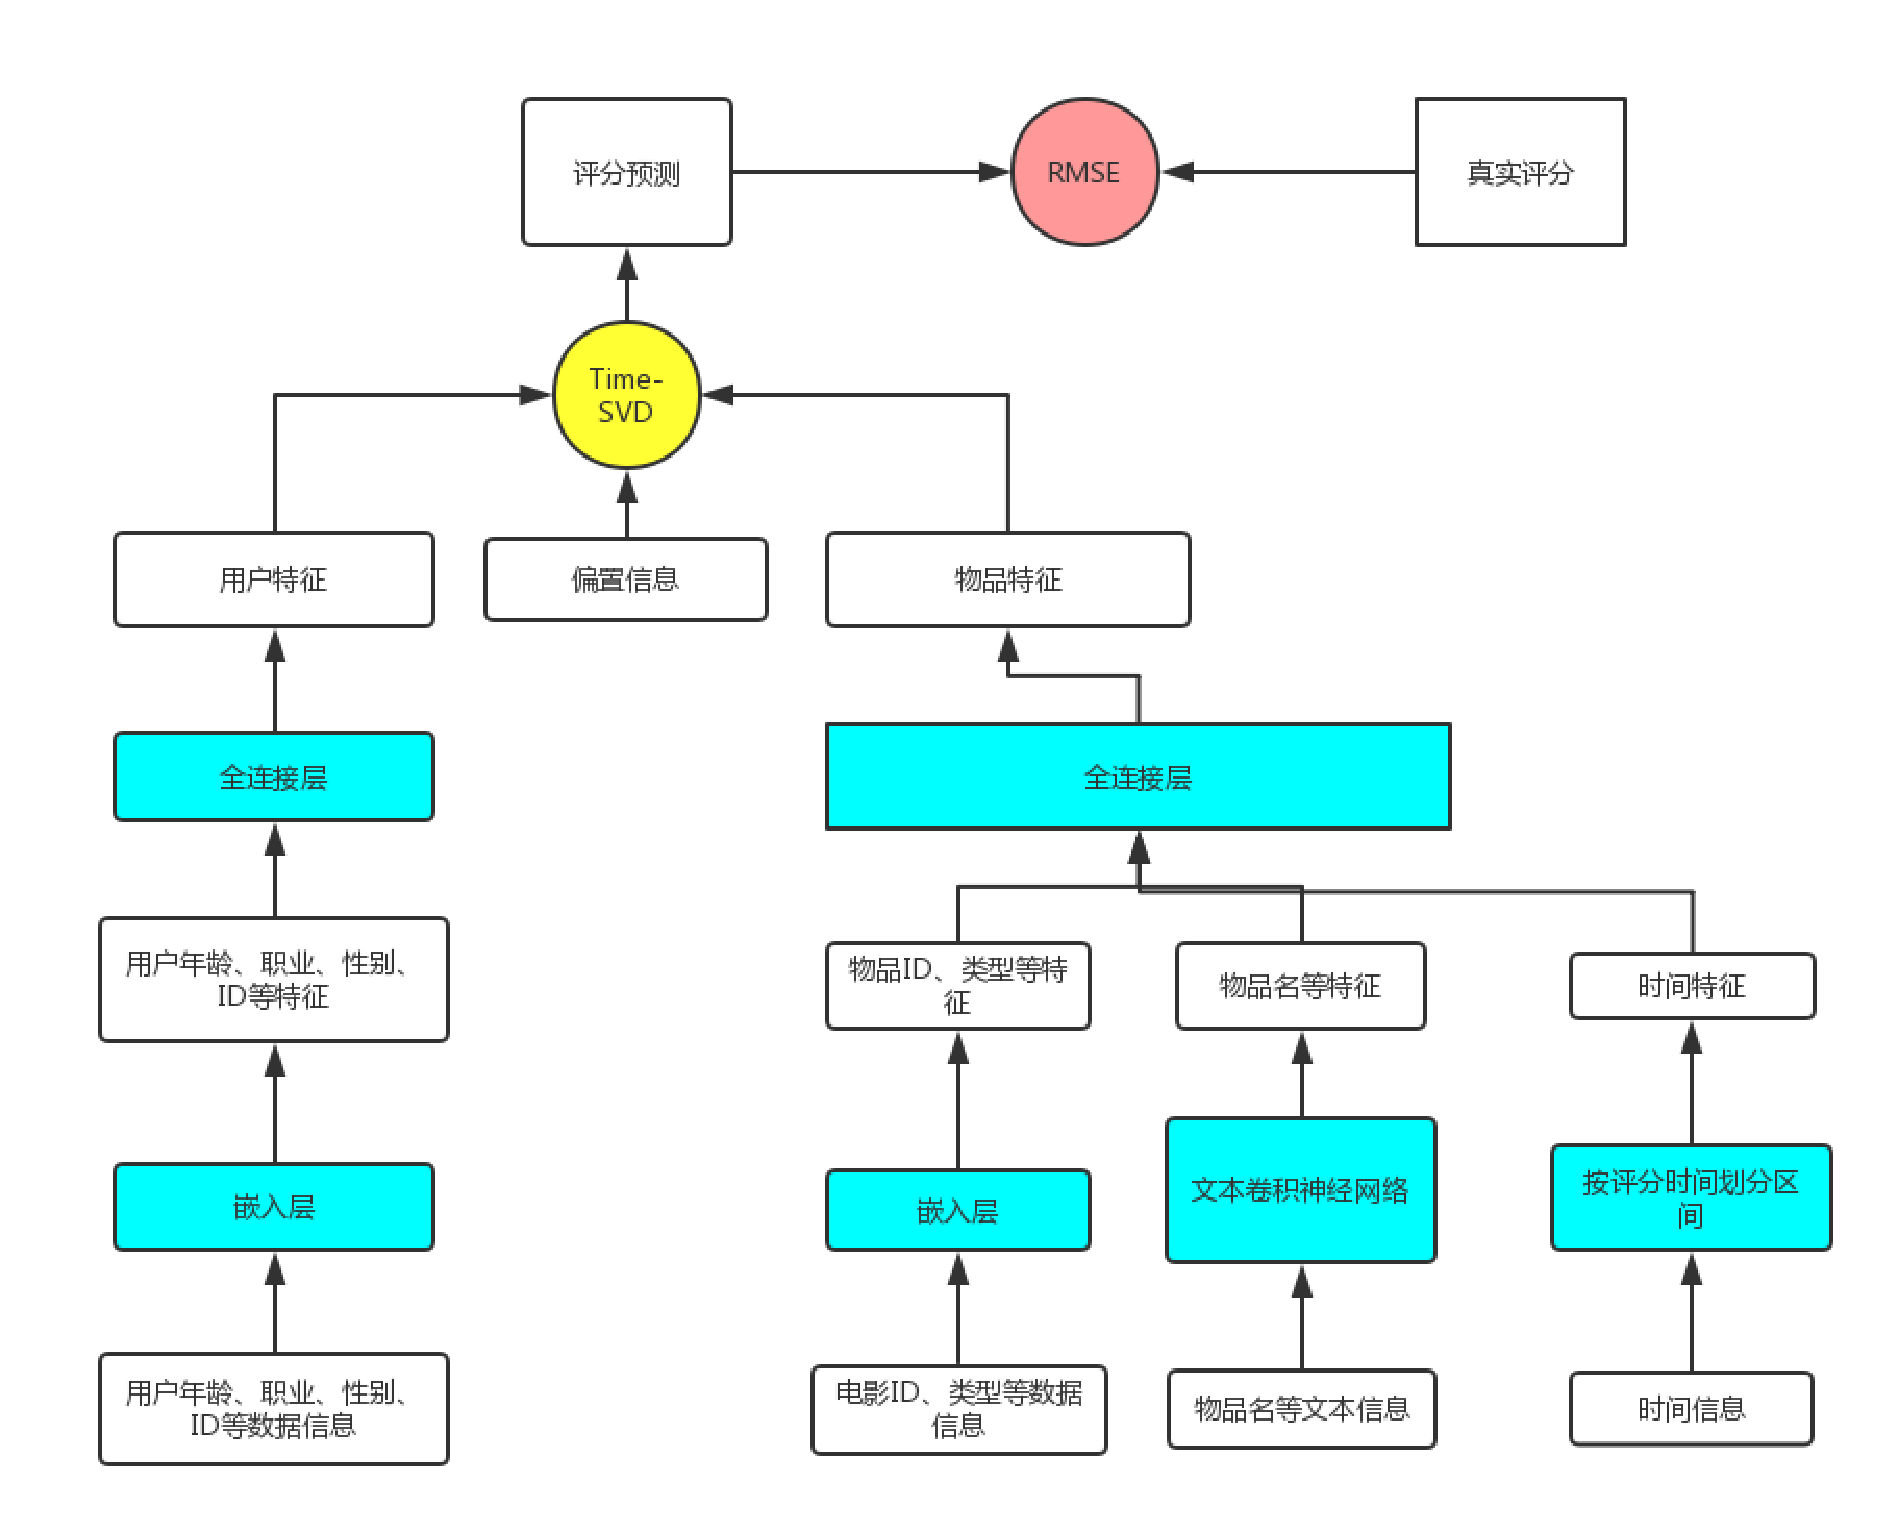
\includegraphics[width=0.8\linewidth]{images/myModel.pdf}
\caption{模型设计示意图}
\label{fig:fig1}
\end{figure}

基于上面所述内容,我们的研究将会在真实的数据集上,首先利用卷积神经网络将用户和物品中稀疏、高维的数据信息转化为稠密低维的特征信息。接下来再结合Time-SVD++的矩阵分解方法,将时间信息考虑进来,并与前面所得到的用户、物品向量一起建模,构建出一种如上图所示的,新型合理的评分预测模型。
\section{研究任务}
在这个背景下,我们的研究大致有如下几项任务:

1)获取并分析原始数据

本次实验我们主要使用MoviLens的1M数据集以及Netflix数据集。MovieLens数据集是由GroupLens通过收集整理电影评分网站MovieLens的评分数据而发布的,1M数据集包含6040个用户和3952部电影,共有1000209个用户评分记录。Netflix数据集则是由在线影片租赁商Netflix举办推荐竞赛时提供的。

2)数据预处理

原始的数据包含很多的类别字段,以电影类别为例就包含犯罪片、动作片、科幻片等不同的类型。为了更方便地处理数据,我们需要使用one-hot编码用数字来代替原始的类别字段。同时我们还需要对原始数据进行去去噪处理来提取关键项的数据。

3)使用卷积神经网络提取数据特征信息
用户部分的处理相对简单,我们需要将用户信息输入嵌入层,从嵌入层索引出特征以后,将特征传入全连接层,从而得到用户特征向量。而物品部分的处理则略有不同,这里我们需要额外使用文本卷积网络来单独处理物品名特征,之后再传入全连接层,与其他信息一起得到物品的特征向量。

4)矩阵分解建模

在建模部分我们借鉴了传统的Time-SVD++的方法,将评论的时间信息划分为不同的区间,利用不同的时间区间分别学习出隐因子向量,从而在建模时加入时间因素。同时我们还需要在建模阶段加入偏置信息,从而使得评分预测结果更具有普遍性。

5)实验和分析
在实验阶段我们需要评估模型在评分预测和top-N推荐方面的表现,并与常见的规范化矩阵奇异值分解(Funk-SVD)、非负矩阵分解(NMF)还有Time-SVD++方法进行比较。

评分预测中,我们使用均方根误差(root-mean-square error,RMSE)来评估预测的误差,其定义如下。

\begin{equation*}
RMSE = \sqrt{  \dfrac   {\sum\limits_{u,i \in T}  (r_{u,i} - \hat{r_{ui}}) ^2 } {|T|}   }.
\end{equation*}

对于测试集中的一个用户 $u$ 和物品 $i$ ,另 $r_{ui}$ 是用户 $u$ 对物品  $i$  的实际评分,而 $\hat{r_{ui}}$  是推荐算法给出的预测评分。

而在top-N推荐方面,我们则使用,命中率(Hit Ratio,HR)和归一化累积获得指标(Normalized Discounted Cumulative Gain,NDCG)来进行评估。

\chapter{技术路线}
\section{文本卷积神经网络(Text-CNN)}
卷积神经网络(CNN)在计算机视觉领域应用广泛,凭借其强大的局部特征捕捉能力,CNN为分析和利用图像数据的研究者提供了极大的帮助。而Yoon Kim等人\cite{Kim14fTextCNN}则将CNN应用到了文本分类中,提出了Text-CNN。在本研究中,Text-CNN被用来学习物品的文本信息,从而获得隐藏层向量。
TextCNN通常由四部分构成:输入层、卷积层、池化层、全连接层,如下图所示:

\begin{figure}[htbp]
\centering
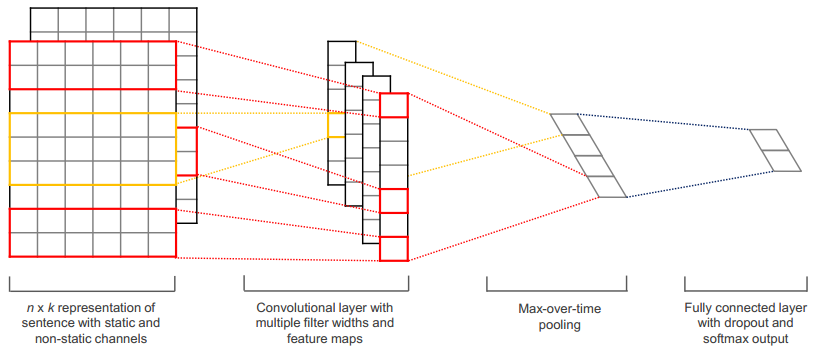
\includegraphics[width=0.8\linewidth]{images/textCNN.png}
\caption{TextCNN结构示意图}
\label{fig:fig2}
\end{figure}



1)输入层

输入层是句子中词向量自上而下排列的矩阵,假如句子中有$n$个词,向量的维数是$k$,那么输入层就是一个$n\times k$的矩阵。
这里,我们用$x_i \in  \mathbb{R}^k$来表示句子中第$i$个$k$维向量。那么一个长度为$n$的句子就可以表示为:

\begin{equation}
x_{1:n} = x_1 \oplus x_2 \oplus ...\oplus x_n
\end{equation}
2)卷积层

在卷积层需要做的一件事就是卷积。卷积操作常用来做图像处理,就是取一定窗口大小的图像矩阵与滤波器(权重矩阵)做内积(逐个元素相乘再相加)。
用数学公式表示就是,用$w \in \mathbb{R}^{hk}$来表示滤波器,那么一个特征$c_i$就是由一个窗口中的词语$x_{i:i+h-1}$所生成:
\begin{equation}
c_i = f(w\cdot x_{i:i+h-1} + b)
\end{equation}
这里$b\in \mathbb{R}$是偏置项,而$f$则是像双曲函数这样的非线性函数。
这里,我们就可以从句子里每$h \times k$的窗口${x_1:h,x_2:h,...,x_{n-h+1:n}}$通过卷积操作得到若干个特征图(Feature Map)
\begin{equation}
c = [c_1, c_2,...,c_{n-h+1}]
\end{equation}

其中$c \in \mathbb{R}^{n-h+1}$

3)池化层

在池化层中,TextCNN采用了一种称为Max-over-time Pooling的方法。该方法从之前得到的一维特征图中提取出最大值:$\hat{c} = \max\{c\}$。因为最大值往往代表着最重要的信号。而同时,因为不管特征图中有多少值,只需提取出其中的最大值,池化操作也可以解决不同长度的句子输入问题。
最终池化层输出的结果为各个特征图的最大值的集合,即一个一维向量。

4)全连接层

在TextCNN中,池化层中的一维向量的输出通过全连接的方式连接到Softmax层中进行分类。而在全连接层中则使用Dropout技术,并对全连接层上的权重参数给予L2正则化的限制,从而防止过拟合的发生。
举例来说,如果我们用$m$来表示滤波器的个数,那么池化层的输出结果就可以用$z = [\hat{c_1},...,\hat{c_m}]$来表示。在正则化阶段,dropout会使用如下方式来优化权重参数$w$
\begin{equation}
y = w\cdot(z \circ r) + b
\end{equation}
这里$\circ$ 是向量按位乘法的操作,而$r\in \mathbb{R}^m$则是由概率值$p$为1的伯努利随机变量所生成的屏蔽向量(masking vector)。

\section{奇异值分解(SVD}

\subsection{基本的奇异值分解}
奇异值分解(SVD)是一种最基本的矩阵分解方式,它的核心思想是认为用户的兴趣只受少数几个因素$k$的影响,因此将稀疏且高维的User-Item评分矩阵分解为两个低维矩阵,如下所示。
\begin{equation}
U_{m\times k}V_{n\times k}^T \approx A_{m \times n}
\end{equation}
这里$m$代表用户数量,$n$代表物品数量,$k$代表选取的特征数量。真实数据集中$m$和$n$的值很大,而$k$相比之下要小很多,至少两个数量级以上。
而要计算物品$i$推荐给用户$u$的推荐分数,则需要计算内积,如下所示。
\begin{equation}
\hat{r_{ui}} = q_i^Tp_u
\end{equation}
其中$p_u$和$q_i$分别为用户$u$和物品$i$的特征向量。
但是大多数真实数据集上的评分矩阵都是相当稀疏的,所以它只关注这些很少的值会导致过拟合问题。早期通过填补矩阵中缺失的评级使矩阵变得稠密,但是随着可见项的增加,计算量可能难以承受,另外,不准确的填充会严重影响预测的效果。可以通过引入正则项缓解过拟合的问题,为了得到特征向量,系统最小化在已知评分上的正则平方误差:
\begin{equation}
\min_{q^*, p^*} {\sum\limits_{(u,i) \in \kappa} {{(r_{u,i}-q_i^Tp_u)}^2 + \lambda(||q_i||^2 + ||p_u||^2)} } ,
\end{equation}
这里,$\kappa$ 是训练集中所有已知评级的用户物品对 $(u,i)$ 的集合,系统通过拟合之前观测的样本来学习模型的参数,而我们的目标是预测未知的评分,所以应该通过正则化参数来避免过度拟合已知的项,常数 $\lambda$ 用于控制正则化的程度。可以通过随机梯度下降或迭代最小二乘的方法最小化上面的式子。


\subsection{带偏置的奇异值分解}

基本的矩阵分解方法通过学习用户和物品的特征向量进行预测,其中用户的特征向量代表了用户的兴趣,物品的特征向量代表了物品的特点。但是我们观测到的评分数据中,有很大一部分与用户对物品的喜好无关而只取决于用户或物品本身的特性。以电影推荐为例,标准宽松的用户往往会给出偏高的评分,而相对严格的用户的评分则普遍偏低;而同样,受大众欢迎的电影,往往会得到偏高的评分,而一些烂片的评分则普遍偏低。
我们把独立于用户或物品的因素称为偏置(Bias)部分,可以用如下公式来表示。
\begin{equation*}
b_{ui} = \mu + b_u + b_i
\end{equation*}

$\mu$是训练集中所有评分记录的全局平均数,它表示了训练数据的总体评分情况。$b_u$是用户偏置,表示某一特定用户的打分习惯。$b_i$是物品偏置,表示某一特定物品得到的打分情况。
接下来进行参数优化,损失函数如下所示:
\begin{equation}
\min_{q^*, p^*} {\sum\limits_{(u,i) \in \kappa} {{(r_{u,i}-\mu-b_u-b_i-q_i^Tp_u)}^2 + \lambda(||q_i||^2 + ||p_u||^2 + b_u^2 + b_i^2)} } ,
\end{equation}
其中参数$q_i$、$p_u$、$b_u$、$b_i$仍然可以采用交替最小二乘或随机梯度下降进行优化。
而加入以上偏置信息的评分预测公式如下所示。
\begin{equation}
\hat{r_{ui}} = \mu + b_u + b_i + q_i^Tp_u
\end{equation}

\subsection{加入时间动态的奇异值分解}
在上面加入偏置信息的基础上,我们仍然需要考虑两个变化性的因素:一方面,每个物品的受欢迎程度$b_i$会随着时间变化而变化;另一方面,用户的评价标准$b_u$也会随时间而发生改变,我们使用如下公式来表示。
\begin{equation}
b_{ui}(t) = \mu + b_u(t) + b_i(t)
\end{equation}
这里$b_{ui}(t)$表明第$t$天用户$u$对物品$i$的基准评价,而$b_u(t)$和$b_i(t)$则是用户和物品偏置随着时间而改变的具体函数值。
这里我们需要对时间按区间划分为时间段,每个时间段内使用一个不同的值。

对于物品来说:
\begin{equation}
b_i(t) = b_i + b_{i,Bin(t)}
\end{equation}
其中$Bin(t)$为时间对应的函数。

而对于用户$u$,我们用$t_u$表示时间的平均值,那么用户打分对于时间$t$的导数$dev_u(t)$可以表示为:

\begin{equation*}
dev_u(t) = sign(t - t_u)\cdot |t - t_u|^\beta
\end{equation*}
这里的$|t - t_u|$是用来衡量时间$t$和$t_u$之间的距离。
于是用户偏好关于时间的偏置信息可以表示为:
\begin{equation}
b_u(t) = b_u + \alpha_u \cdot dev_u(t)
\end{equation}
新的损失函数为:
\begin{equation*}
\min_{u, i, t} {\sum\limits_{(u,i) \in \kappa} {{(r_{u,i}(t)-\mu-b_u - \alpha_udev_u(t)-b_{u,t}-b_i - b_{i,Bin(t)}}^2 + \lambda(b_u^2 + \alpha_u^2 + b_{u,t}^2 + b_i^2 + b_{i,Bin(t)}^2))}} 
\end{equation*}

于是我们得到了将用在本次研究的评分预测公式:
\begin{equation*}
\hat{r_{ui}} = \mu + b_u(t) + b_i(t) + q_i^Tp_u(t)
\end{equation*}
\chapter{可行性分析}
1)数据可行性

互联网的飞速发展在改变人们生活方式的同时,也将用户的行为数据保存了下来。不管是用户显示的打分数据,还是点击、浏览商品时产生的隐式反馈数据,这其中都蕴含着丰富的潜在信息,来等待商家还有研究者进行挖掘。而这也为推荐系统领域的相关研究带来了广泛而多样的数据集。

以我们本次所将使用的MovieLens数据集为例,其中就包含用户数据users.dat,电影数据movies.dat还有评分数据ratings.dat。其中的用户数据包含用户ID、性别、年龄、职业和邮编等,这些数据可以在研究中用来学习用户的特征向量,电影数据中的ID、风格则可以用来学习物品的特征向量,其中的电影名作为文本信息则可以利用TextCNN来进行处理。而评分数据中的时间戳字段则可以用来发现用户的兴趣漂移规律,其中的评分数据则可以分成训练集和测试集,分别用来优化参数和评估模型的实际效果。

2)环境可行性

当前推荐系统的研究依然火热,从最早的Netflix电影推荐大赛,KDD Cup数据挖掘竞赛,再到前段时间的阿里移动推荐大赛,京东的JData算法大赛。用于改进推荐算法的竞赛层出不穷,各家平台甚至拿出不菲的奖金来鼓励参赛者对自己现有的推荐算法进行改进。由此可见,在当前外部环境研究推荐算法的改进策略是顺势而为,大势所趋。

3)技术可行性

虽然在推荐系统领域,深度学习还处于一个新兴的阶段。但其在文本处理等方面的成功应用,也为其在挖掘用户和物品的关联信息等方面提供了借鉴。而谷歌推出的TensorFlow,Facebook推出的pytorch,当下也已经成为应用非常广泛的深度学习框架,方便研究者进行深度学习方面的研究。而前面提到的Time-SVD++和TextCNN技术都已经在相应数据集上跑出了不错的效果,其学习过程均可收敛从而达到最优解。由此可见,本次基于深度学习的矩阵分解算法研究具有较高的技术可行性。

4)经济可行性

我们本次使用的均是平台上公开的真实数据集,且仅用于研究,而非处于商业目的。且研究过程主要依赖软件来实现,同时实验所在的浙大电子服务研究中心也已经配备了装有Tesla K40c GPU的服务器,可以用于加速接下来深度学习实验的进行。
\chapter{预期目标及研究计划进度安排}

\section{预期目标}

本次的推荐算法研究,旨在利用卷积神经网络来挖掘数据中的隐含关联信息,并结合矩阵分解,融合时间信息因素,提出一种合理的推荐算法模型,并希望能在RMSE等评分预测指标以及HT、NDCG等衡量top-N推荐质量的指标上,相比于传统的矩阵分解模型有一定程度的改进,缓解推荐时常遇到的数据稀疏和冷启动问题。
\section{进度安排} 
根据之前所述的研究方法和预期结果,将论文的进度计划安排如下:

\begin{table}[h]
\centering
\label{my-label}
\begin{tabular}{cc}
\hline
\rowcolor[HTML]{EFEFEF} 
\textbf{时间}           & \textbf{进度安排}                \\ \hline
2017.7 - 2017.12      & 阅读相关文献资料,充分理解现有的研究成果,并撰写文献综述 \\ \hline
2018.3.1 - 2018.3.20  & 提出初步的研究方案,与导师进行讨论,做出补充和改进    \\ \hline
2018.3.21 - 2018.4.1  & 根据研究方案确定初步的模型,并撰写开题报告                \\ \hline
2018.4.2 - 2018.4.10 & 获取实验数据,分析数据并进行预处理            \\ \hline
2018.4.11 - 2018.4.25 & 实现论文中的关键算法,并在数据集上测试效果        \\ \hline
2018.4.26 - 2018.5.5 & 对比不同算法,并对各项指标进行分析            \\ \hline
2018.5.6 - 2018.5.15 & 对研究结果进行归纳,整理实验数据,完成论文初稿      \\ \hline
2018.5.15 - 2018.5.30  & 完善和修改,并确定论文终稿                \\ \hline
\end{tabular}
\end{table}



\bibliography{data/kaiti}








  %!TEX root = ../main.tex


\centerline{\textbf{\xiaoer{本科毕业论文文献综述}}}
\bigskip

\textbf{摘要}\quad 
随着互联网的飞速发展,用户在线上所接触到的信息在复杂性和多样性等方面呈现出爆炸性增长的趋势。而推荐系统作为解决信息过载问题的一个切实有效的办法,在人们的日常生活中扮演着越来越重要的角色。同时,近些年来,深度学习在语音、图像还有自然语言处理等方面所取得的革命性的进展也越来越受到人们的关注。而相关的研究也表明:深度学习在信息检索和推荐等方面同样也有不错的表现。特别是亚马逊、YouTube等将深度学习应用到了自己网站的推荐系统上\cite{CovingtonAS16YouTube},并且取得了很好的效果。而这些也使得利用深度学习改进现有推荐算法成为当下研究的一个热点。
本文旨在在传统推荐方法的基础上,讨论推荐系统所面临的常见问题,以及深度学习在这些问题上的一些富有成果的研究,并对涉及到的相关深度学习技术进行具体的解释。


\chapter{背景}
在信息爆炸性增长的今天,个性化推荐系统已经成为人们生活中必不可少的筛选利器,并以多种多样的形式影响着人们生活的方方面面:亚马逊、淘宝等电商网站利用推荐引擎实时提供用户可能感兴趣的商品推荐;Twitter、Facebook等社交网站利用推荐系统为用户寻找潜在的好友推荐;Yotube、优酷等视频网站在用户观看视频的同时,利用推荐系统为用户提供最可能点击的视频推荐;Quora、今日头条等新闻门户网站则利用推荐系统帮用户筛选出最有价值的新闻。互联网广告利用推荐系统准确的找到潜在客户群,相比于随机投放提高了效率。推荐系统在促进商业发展以及便利人们决策等方方面面发挥着越来越重要的作用。

通常来说,推荐的内容列表一般是根据用户偏好、物品特征、用户与物品交互的历史记录以及一些诸如时间和空间数据这样的辅助信息而生成的。推荐系统的模型主要可以分为基于协同过滤的推荐、基于内容的推荐以及基于不同输入数据的混合推荐\cite{AdomaviciusT05}。然而这些模型在解决数据稀疏性(用户已评分的物品占总物品数量的很少一部分),冷启动问题(新的用户和新的物品往往没有评分数据)以及如何权衡不同指标下的推荐效果等问题上都有其各自的局限性。\cite{AdomaviciusT05}\cite{VekariyaK12Hybrid}\cite{McNeeRK06Being}\cite{VargasC11Rank}

在过去的十年间,我们已经见证了深度学习(Deep Learning)在诸如计算机视觉以及语音识别等领域的应用上,取得了显著的成功。而深度学习在解决很多复杂任务的良好效果,也促使学术界和工业界争相将其应用到其他更广阔的领域。最近,深度学习已经被逐渐应用到了推荐系统上\cite{CovingtonAS16YouTube}\cite{ChengKHSCAACCIA16Wide&Deep},改变了传统推荐系统的架构,并且在提升用户体验和满意度方面取得了令人瞩目的效果。一方面,通过学习一种深层次的非线性网络结构,深度学习可用来表征用户和物品相关的海量数据,利用这种强大的从样本中学习数据集本质特征的能力,可以获得用户和物品的深层次的特征表示。而另一方面,深度学习还能从诸如上下文、文本、图像等繁杂的数据中提取出数据之间错综复杂的内在关系,从而将不同数据映射到一个相同的隐空间,能够获得数据的统一表征\cite{PengZZXHLZHG17Cross-Media},在此基础上结合传统推荐方法来做推荐,可以有效利用多源异构数据,缓解传统推荐系统中的数据稀疏和冷启动问题。

推荐系统是工业领域中必不可少的一部分,在许多在线网站和手机应用中都为提升销量和服务发挥着不可忽视的作用。举例来说,人们在Netflix()中所观看的影片有$80\%$是来自于推荐\cite{Gomez-UribeH16Netflix},在YouTube上的视频点击有60\%是来源于推荐\cite{DavidsonLLNVGGHLLS10Youtube}最近,像Netflix、YouTube这样的公司也借助深度学习来提高推荐的质量\cite{ChengKHSCAACCIA16Wide&Deep}\cite{CovingtonAS16YouTube}\cite{OkuraTOT17Embedding}。比如Covington等人就提出了一种应用在YouTube上的借助于深度神经网络的视频推荐算法\cite{CovingtonAS16YouTube}。Cheng提出了一种应用在Google play App上的深广学习(wide\&deep)模型\cite{ChengKHSCAACCIA16Wide&Deep}。Shumpei则提出了一种应用在Yahoo新闻上的基于RNN的新闻推荐系统\cite{OkuraTOT17Embedding}。这些模型都已经在线上进行了测试,并且可以大幅度提高传统模型的推荐性能。可以预见的是,深度学习将引领推荐系统领域的一次巨大变革。

另一项令人瞩目的改变则发生在学术研究领域。近些年,基于深度学习的推荐算法的论文数量呈现出几何倍数的增长。
作为推荐系统领域的顶级会议,ACM推荐系统年会(ACM RecSys),在2016年就专门召开了第一届基于深度学习的推荐系统研究专题研讨会(DLRS'16),旨在促进基于深度学习的推荐系统在学术研究和工业应用的发展。由此可见,基于深度学习的推荐系统研究已经成为研究推荐系统的热点方向之一。

总而言之,不管是在学术研究还是工业应用,深度学习在推荐领域都已经取得了令人振奋成果。而要想在这一领域继续有所突破,理解和归纳前人研究模型的优缺点,必然是不可缺少的一项工作,而这也正是本文写作的目的所在。



% chapter 背景(end)

\chapter{传统推荐系统}
自从20世纪90年代,协同过滤技术被首次提出,推荐系统已经成为了一门独立的学科而受到了广泛的关注。作为推荐系统的核心,推荐算法主要是利用用户与物品之间的二元关系,基于用户历史行为记录或相似性关系来帮助发现用户可能感兴趣的项目。文献\cite{AdomaviciusT05}给出了推荐算法的形式化定义:用$U$表示所有用户(user)的集合,用$I$来表示所有物品(item)的集合。在真实系统中,$U$和$I$的规模通常非常大。这里我们定义一个效用函数$s$,用来计算物品$i$对用户$u$的推荐度,即$s:U \times I \rightarrow R$,其中$R$是一个全序的集合,而推荐算法所研究的主要问题就是通过推荐度的计算,为每一个用户$u \in U$找到最感兴趣的物品$i^{'} \in I$,如下所示:
\begin{equation}
\forall u \in U, i_u^{'} = arg \max_{i \in I} s(u,i)
\end{equation}		
在推荐系统领域,我们所需要解决的一个关键问题是如何将效用函数$s$从$U \times I$的一个子空间外推到整个$U \times I$空间。一般来说,我们用用户对物品的评分来表示推荐度,而在真实的推荐系统中,用户往往只评分了其中的一小部分项目。因此,在推荐给用户最感兴趣的物品之前,必须先根据已知评分对未知评分进行预测,这就是我们之前所说的外推过程。根据对未知评分预测方法的不同,传统的推荐算法通常可以分成以下三种\cite{VerbertMOWDBD12ContextAware}:基于内容的推荐(content-based recommendation)、协同过滤推荐(collaborative filtering recommendation)和混合推荐(hybrid recommendation)。
\section{主要算法介绍}
\subsection{基于内容的推荐}
基于内容的过滤方法为每个用户或物品创建描述以表征其性质,例如,电影的描述可以包括其类型、导演、票房等方面,用户的描述可以是个人资料或从已评分物品中识别出的共同特征。这样就能计算出用户与待测物品在内容上的匹配度,进而根据匹配度对所有需要预测的物品进行排序,最终为用户推荐其潜在感兴趣的物品。
% subsection 基于内容的推荐(end)
\subsection{协同过滤推荐}
协同过滤利用相似用户之间具有相似兴趣偏好的规律,来发现用户对物品的潜在偏好。举个例子来说,基于用户的协同过滤算法(User-based Collaborative Filtering)会搜索那些与目标用户具有相似评分模式的用户作为相似用户,然后利用这些兴趣相投的相似用户的评分来预测其他未评分物品的评分。而基于物品的协同过滤算法(Item-based Collaborative Filtering)则是从物品的角度出发来预测评分。它首先计算一个物品-物品的相似矩阵,来确定每一对物品之间的相似度。然后再根据目标用户对相似物品已有的评分,来预测目标用户对未评分产品可能的评分。
% subsection 协同过滤推荐(end)
\subsection{混合推荐}
混合推荐通过组合不同推荐算法,往往能相比单一推荐算法,产生更好的性能。举例来说,可以以协同过滤算法为框架,结合基于内容的推荐算法来环节数据稀疏问题,这属于模型层面上的混合推荐。也可以将所有用户属性、用户行为等数据作为输入,通过训练一个统一的分类器来产生推荐结果,这属于特征层面上的混合推荐。
% subsection 混合推荐(end)
% section 主要算法介绍(end)
\section{传统算法存在的问题}
协同过滤算法是目前应用最为广泛的推荐算法,但往往面临数据稀疏和冷启动等问题。此外,经典的协同过滤算法采用的浅层模型往往无法学习到用户和物品更深层次的特征。基于内容的推荐算法可有效缓解数据稀疏和新物品的冷启动问题,但相应的,这种算法依赖于有效的特征提取,而传统的浅层模型往往需要人工设计特征,其有效性和可扩展性非常有限。近些年来,蕴含用户丰富个性化需求信息的文本、图像、标签在内等多源异构数据被越来越多地加入到了传统的推荐算法中。而融合了多源异构辅助信息(side information)的混合推荐算法也越来越被人们所重视,在解决数据稀疏和冷启动问题上具有不错的效果。但是由于辅助信息往往具有多模态、数据异构、大规模、数据稀疏和分布不均匀等复杂特征,融合多源异构数据的混合推荐方法研究依然面临着严峻的挑战\cite{WangWY15CDL}\cite{ZhangYLXM16CKBE}。
% section 传统算法存在的问题(end)
% chapter 传统推荐系统(end)

\chapter{基于深度学习的推荐系统}
\section{深度学习技术}
深度学习属于机器学习的一个子领域,它从数据中学习到不同层次的数据表示和抽象,可以用来解决有监督和无监督学习任务\cite{DengY14DLMA}。本节中,我们主要介绍一些和推荐系统领域密切相关的深度学习技术。

\subsection{多层感知机(Multilayer Perceptron, MLP)}
多层感知机(MLP)是一种前馈神经网络,与传统的只有输入层和输出层的感知机不同,它在输入和输出层之间加入一个或多个隐藏层。因此,多层感知机可以灵活应用激活函数(activation function)使其不仅仅局限于二分类问题。

这里以一个最简单的只含有一个隐藏层的MLP为例\cite{abs-1801-07883DLS}:
\begin{figure}[h]
\centering
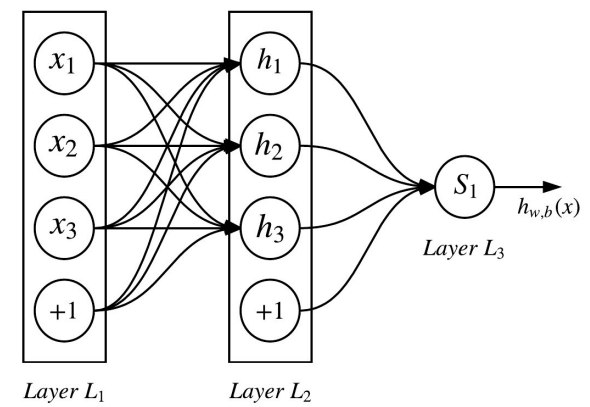
\includegraphics[width=0.5\linewidth]{images/MLP.png}
\caption{只含有一个隐藏层的MLP}
\label{fig:fig1}
\end{figure}
我们用一个$3$维向量$X=[x_1,x_2,x_3]$表示图中输入层,用$3$维向量$H[h_1,h_2,h_3]$表示图中隐藏层.则有$H = f(W^{T}X) = f(\sum\nolimits_{i=1}^{3}W^{1}_{i}x_{i} + b^{1})$其中$W^{1}$是第一层的$3 \times 3$的权重矩阵,$f$是激励函数,$b^{1}$是第一层的偏置项(bias)。这里激励函数$f$通常是非线性的,一般选用$sigmoid$函数、$tanh$函数或者$ReLU$函数。代入之后,表达式分别如下所示:
\begin{equation}
f(W^TX) = sigmoid(W^TX) = \frac{1}{1+exp(-W^TX)}
\end{equation}

\begin{equation}
f(W^TX) = tanh(W^TX) = \frac{e^{W^TX} - e^{-W^TX}}{e^{W^TX} + e^{-W^TX}}
\end{equation}

\begin{equation}
f(W^TX) = ReLU(W^TX) = \max(0,W^TX)
\end{equation}
而由隐藏层到输出层则可以看成是一个多类别的逻辑回归,一般选用$softmax$函数作为激励函数。则输出可以表示为$softmax(\sum\nolimits_{i=1}^{3}W^{2}_{i}x_{i} + b^{2})$,这里$W^{2}$是第二层的$3 \times 3$的权重矩阵,$f$是激励函数,$b^{2}$是第二层的偏置项(bias)。
总结起来,这个三层MLP用公式总结起来就是
\begin{equation}
g(X) = G(b^{2} + W^{2}(f(b^{1} + W^{1}X)))
\end{equation}
其中函数$G$就是softmax函数,它将多个神经元的输出映射到(0,1)区间内,一般用来进行多分类。$softmmax$函数定义如下:
\begin{equation}
G(X)_j = \frac{e^{x_j}}{\sum\nolimits_{k=1}^{K}e^{x_k}}	\qquad  for \quad j = 1,...,k
\end{equation}
这里$K$代表输入变量$X$的维度。
\subsection{自动编码器(Autoencoder,AE)}
自动编码器依靠编码和解码过程来重构输入数据,从而学习数据的隐层表示。传统的自动编码器可以视为一个三层的神经网络:包含有相同规模的输入层$x$和输出层$y$,还有一个隐藏层$h$,其结构如下图所示。

\begin{figure}[htbp]
\centering
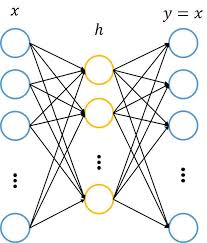
\includegraphics[width=0.22\linewidth]{images/AE.jpg}
\caption{自动编码器结构示意图}
\label{fig:fig2}
\end{figure}

自动编码器的目的是使得输入$x$和输出$y$尽可能接近,并用重构误差来表示这种接近程度。一般重构误差包括均方误差(mean-square error, MSE)和交叉熵(cross-entropy)。
为了解决自动编码器容易学习到一个恒等函数的问题,研究者后来又提出了稀疏自动编码器和降噪自动编码器。2007年,Bengio等人\cite{VincentLBM08Bengio}通过堆叠多个降噪自动编码器,提出了栈式降噪自动编码器(Stacked Denoising Autoencoder, SDAE)的概念。
如今,自动编码器,特别是栈式降噪自动编码器,在推荐系统中主要被用于学习用户和项目的隐层表示,通过重构学习用户和物品的相关信息(如评分数据和文本、图像信息),从而获得用户或物品的隐层表示,最后基于这种隐层表示来预测用户对物品的偏好,并应用在评分预测、文本推荐和图像推荐等场景中\cite{WangSY15SDAE}。
\subsection{卷积神经网络(Convolutional Neural Network,CNN)}
卷积神经网络是当今图像识别领域的研究热点。相比于传统的MLP,卷积神经网络使用池化(pooling)可以减少模型中的神经元数量。特别是当输入层是多维图像的时候,CNN可以将图像直接作为网络的输入,从而可以避免传统处理算法中复杂的特征提取和数据重建过程。卷积神经网络的基本结构主要分为输入层、卷积层、下采样层(池化层)、全连接层和输出层,如下图所示。

\begin{figure}[htbp]
\centering
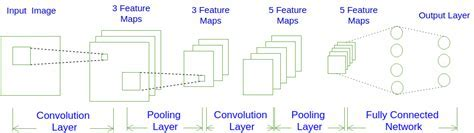
\includegraphics[width=0.5\linewidth]{images/CNN.jpg}
\caption{卷积神经网络结构示意图}
\label{fig:fig3}
\end{figure}

在推荐系统领域,CNN主要被用来从文本、图像、音频等内容中提取物品的隐藏特征,从而获取物品的低维向量表示,其在音乐推荐、图像推荐还有文本推荐等领域都有所应用\cite{GengZBC15IMAGE}。
\subsection{循环神经网络(Recurrent Neural Network,RNN)}
传统CNN的层与层之间是全连接的,而每一层的节点之间则没有连接。与之不同的是,循环神经网络在网络各隐层的节点之间加入连接,从而能够通过获取输入层的输出和前一时刻的隐层状态来计算当前时刻隐层的输出,也就是说RNN能够对过去的信息进行记忆。下图是一个包含输入单元、输出单元和隐层单元的典型RNN结构。

\begin{figure}[htbp]
\centering
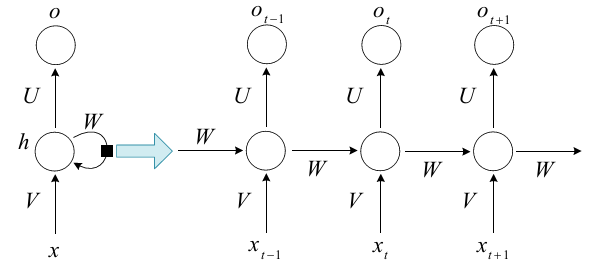
\includegraphics[width=0.5\linewidth]{images/RNN.png}
\caption{循环神经网络结构示意图}
\label{fig:fig4}
\end{figure}

而为了解决传统RNN存在梯度消失和难以学习数据之间的长期以来关系的问题,Hochreiter等人\cite{HochreiterS97LSTM}提出了长短时间记忆网络(Long Shor-Term Memory, LSTM),Cho等人\cite{ChoMBB14GRU}则提出了门限循环单元(Gated Recurrent Unit,GRU)。LSTM和GRU通过增加保存长期状态的隐层单元,能够更加有效地建模长期以来关系,是目前应用最为广泛的循环神经网络模型。
在推荐系统领域,RNN主要用来建模数据之间的序列影响,从而帮助获取更为有效的用户和物品隐层表示。一方面,RNN可以被用来建模推荐系统中用户行为的序列模式\cite{WuABSJ17RRN}\cite{SongEH16DL4TR},另一方面,它还可以被应用在建模用户和物品相关的文本信息中词语之间的序列影响\cite{0014SY16CRA}\cite{0014SY16CRA}。在文本推荐、图像推荐、评分预测以及基于未知社交网络中的兴趣点推荐等领域应用广泛。
\subsection{受限制玻尔兹曼机(Restricted Boltzmann Machine,RBM)} 
玻尔兹曼机(Boltzmann machine, BM)由一些二元的可见单元(对应可见变量,即数据样本)和一些二元的隐层单元(对应隐层变量)构成。当处于状态0,表示该神经元处于抑制状态,而状态1则对应表示该神经元处于激活状态。虽然BM具有强大的无监督学习能力,但其训练过程却非常耗时。为此,Sejnowski等人提出了受限制玻尔兹曼机(Restricted Boltzmann Machine, RBM),通过在原有BM基础上除去同层变量之间的连接,可以显著提高学习效率。
如下图所示,RBM包括可见层$v$以及隐层$h$,两层之间是全连接的,而同层的节点之间则是互不连接的。

\begin{figure}[htbp]
\centering
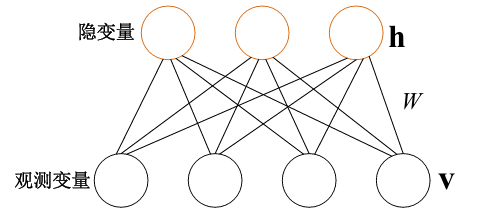
\includegraphics[width=0.5\linewidth]{images/RBM.png}
\caption{受限制玻尔兹曼结构示意图}
\label{fig:fig5}
\end{figure}

作为最早被应用在推荐系统中的神经网络模型\cite{MelloZS07aRBMCF}\cite{TruyenPV09BMCF},RBM当前主要用来重构用户的评分数据,从而学习到用户的隐层表示,进而实现对未知评分的预测。
% section 深度学习技术(end)

\section{深度学习在推荐领域的研究现状}
深度学习当前在推荐系统中,主要用来学习用户和物品的输入数据从而获得隐层表示,然后再根据这种隐层表示为用户推荐物品。一个基于深度学习的推荐系统框架,如下图所示通常包含三层:输入层、模型层还有输出层。

\begin{figure}[htbp]
\centering
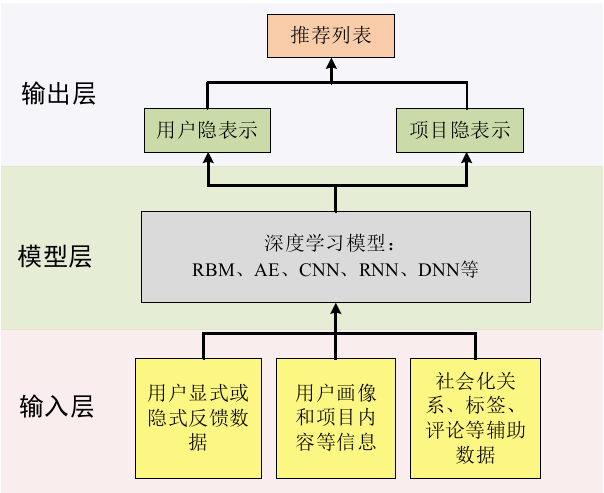
\includegraphics[width=0.5\linewidth]{images/DLframework.png}
\caption{基于深度学习的推荐系统框架}
\label{fig:fig1}
\end{figure}

输入层的数据一般包括:用户的显式反馈(评分、喜欢或不喜欢)或隐式反馈数据(浏览、点击等行为数据)、用户画像(性别、年龄、偏好等)和物品内容(文本、图像等信息)、用户生成内容(社会化关系、标签、评论等辅助数据)。在模型层,通常使用前面提到的深度学习技术(如受限制玻尔兹曼机、自动编码器、卷积神经网络、循环神经网络等)来处理输入数据并获得隐层表示。而在输出层,则将得到的隐层表示通过内积(inner product)、Softmax、相似度计算等方法产生项目的推荐列表。

\subsection{深度学习在基于内容的推荐系统中的应用}
在基于内容的推荐系统中,深度学习可以用来从项目的内容信息中提取物品的隐层表示,以及从用户的画像信息以及历史行为数据中获取用户的隐层表示,之后再基于获得的隐层表示来计算书用户和物品的匹配度,进而为用户推荐物品。

1)基于MLP的内容推荐

Cheng等人\cite{ChengKHSCAACCIA16Wide&Deep}通过学习用户特征、物品特征和情境特征等多源异构数据,提出了用于APP推荐的深广学习(Wide\&Deep Learning)模型。如下图所示,该模型联合训练了一个宽广线性模型(图中左侧)和一个深度神经网络(图中右侧)来确保模型记忆能力和泛化能力的均衡。

\begin{figure}[htbp]
\centering
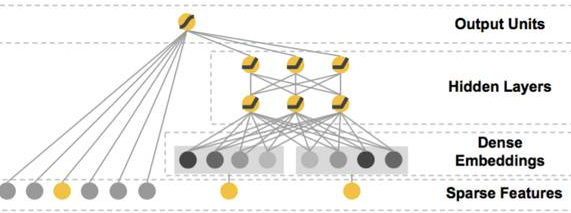
\includegraphics[width=0.5\linewidth]{images/WideDeep.png}
\caption{深广学习模型结构}
\label{fig:fig1}
\end{figure}

与深广模型类似,He等人\cite{abs-1708-05031NCF}提出了一种神经协同过滤方法(Neural Collaborative Filtering,NCF),该方法通过将用户和物品的的特征作为输入,并利用多层神经网络来学习用户和物品之间的交互函数,得到一种矩阵因子分解的泛化结构和一种多层感知机结构。接下来利用神经矩阵因子分解模型(Neural Matrix Factorization Model,NeuMF)来组合矩阵因子分解的线性特征和深度神经网络的非线性特征。除此之外,Covington等人\cite{CovingtonAS16YouTube}也提出了一种基于MLP的深度神经网络模型,并应用在了YouTube视频推荐上。

2)基于CNN的内容推荐

Gong等人\cite{GongZ16HashtagAttention}提出了一种基于注意力的卷积神经网络(Attention-based Neural Network)来进行微博中的Hashtag推荐。这里,作者将hashtag推荐问题理解为一个多标记分类问题,并用CNN来获取微博的特征。之后,Zhang等人\cite{ZhangWHHG17HashtagMulti}通过利用多模信息来进行微博的hashtag推荐。这里,作者采用CNN从图像中提取特征,而用RNN从文本中提取特征,之后再结合这两方面的特征来进行标签推荐。而注意力机制则用来建模图像和文本信息的局部关联性。除此之外,Wang等人\cite{WangYRTZYW17ArticleRec}则利用CNN来学习文章中的语义信息,提出了一种动态注意力深度模型(Dynamic Attention Deep Model,DADM),用来研究编辑者的文章推荐问题。Oord等人\cite{OordDS13MusicRec}则利用CNN来学习音乐的音频信号数据和用户的历史收听数据,来解决音乐推荐系统中的冷启动问题。

3)基于RNN的内容推荐

与基于注意力的CNN模型类似,注意力机制也被用于基于RNN的内容推荐中。Li等人\cite{LiLJZ16HashtagRNN}就提出了一种基于注意力的LSTM模型来进行微博中的hashtag推荐。将RNN与注意力机制结合起来,可以帮助提取文本中的序列特征,从而在微博中识别出最具有信息量的词。同时,RNN还经常被用来做新闻推荐,Okura等人\cite{OkuraTOT17NewsRecRNN}就首先使用降噪自动编码器(DAE)来从新闻中提取出文章的隐层表示,并采用RNN来从用户的历史行为列表中来学习用户的隐层表示,从而来获取用户偏好,之后将基于新闻和用户的隐层表示用点乘进行关联,最终为用户产生新闻推荐列表。

\subsection{深度学习在协同过滤中的应用}
将深度学习应用于协同过滤中,可有效改善传统矩阵因子分解可扩展性不足的问题\cite{SalakhutdinovMH07RBM}。其通常做法一般是,将用户的评分向量(或者是物品的被评分向量)作为输入,利用深度学习来学习用户或物品的隐层表示,之后再利用逐点损失(Point-wise Loss)和成对损失(Pair-wise Loss)等损失函数来对模型的参数进行优化\cite{WuDZE16CDAE},最后再用学习到的隐层表示来进行物品推荐。

1)基于AE的协同过滤

自动编码器近些年来,被越来越多地应用到了传统的协同过滤方法中。如Sedhain等人\cite{SedhainMSX15AECF}提出的基于自动编码器的协同过滤模型(AutoRec),就利用自动编码器的编码过程和解码过程来产生输出,并通过最小化重构误差来优化模型的参数,进而对评分进行预测。而与AutoRec不同的是,Strub等人\cite{CFSDAE}利用两个栈式降噪自动编码器(SDAE),针对评分矩阵的稀疏性问题,在训练过程中直接将评分矩阵中的缺失值归零,从而减少了网络的连接数量。Wu等人\cite{WuDZE16CDAE}的协同降噪自动编码器(Collaborative Denoising Auto-Encoders,CDAE)则是将自动编码器应用到了top-N推荐问题上。

2)基于RBM的协同过滤

Salakhutdinov等人\cite{TruyenPV09BMCF}在2007年最早将受限制玻尔兹曼机应用到协同过滤推荐模型之中。针对传统RBM模型仅仅利用物品之间的关联关系,Georgiev等人\cite{GeorgievN13NONIID}在原有RBM模型基础上进行了扩展,并且简化了模型的训练和预测过程。后来,何洁月等人\cite{HeJieYue}又将好友信任关系加入到RBM之中,提出一种基于实值状态的玻尔兹曼机,有效缓解了原有模型的稀疏性问题。

3)基于RNN的协同过滤

RNN能够建模用户行为之间的相互依赖关系,也可以用来建模用户的历史行为对当前时刻用户行为的影响。因此可以利用RNN,在传统协同过滤之中融入时间序列信息,从而提升推荐系统的性能。为此,Song等人\cite{SongEH16DL4TR}通过融入时间信息并在多种粒度上建模用户的兴趣偏好,提出了一种多等级时间深度语义结构化模型(Mutli-Rate TDSSM)。而考虑到推荐系统中的用户行为之间往往存在着多种类型,Liu等人\cite{LiuWW17RLBL}提出了一种循环Log双线性模型(Recurrent Log-BiLinear,RLBL),该模型用RNN来建模用户行为之间的长程依赖关系,而用Log双线性模型(Log-BiLinear,LBL)\cite{MnihH07LBL}来建模短时的情境信息,从而对用户在下一时刻的行为信息进行预测。

\section{基于深度学习的推荐系统的优势和存在的问题}
基于深度学习的推荐系统能够有效地融合多源异构数据,可以缓解传统推荐系统中的数据稀疏和冷启动问题。而融合多种推荐方法的混合推荐,虽然也可以在一定成都上缓解数据稀疏问题,但是这种方法却面临着辅助数据难以表示的问题。传统的方法,如协同主题回归(Collaborative Topic Regression,CTR)\cite{WangB11CTM},并不能获取辅助数据的有效表示\cite{WangWY15CDL}。而利用深度学习来自动提取特征,则可以从辅助数据中学习到有效的用户和物品隐层表示。
\subsection{优势}
总的来说,相比于传统推荐方法,基于深度学习的推荐方法一般有以下三点优势:

1)传统浅层模型提取到的特征通常是稀疏和高维的,而深度学习可以学习到非线性的多层次抽象特征表示,获取稠密和低维的特征表示\cite{ChengKHSCAACCIA16Wide&Deep}。

2)深度学习可以克服不同数据之间的异构性\cite{ZhangYLXM16CKBE}\cite{CovingtonAS16YouTube},可以方便地通过各种粗糙的原始数据的输入来学习到用户和物品的隐层表示。

3)深度学习可以帮助从图像、视频这样的非结构化中提取特征信息,避免复杂的人工特征工程\cite{ZhangYLXM16CKBE}。
\subsection{存在的问题}
同时,基于深度学习的推荐方法往往也存在着以下问题:

1)可解释性问题。基于深度学习的推荐模型往往类似于一个黑盒,难以为最终做出的推荐结果找到一个合理的解释。而如何在增强深度学习在推荐系统中的可解释性,仍需要进一步的深入研究。

2)可扩展性问题。深度学习在推荐系统中的另一个难题在于,其模型往往需要长时间的训练,而权衡模型的可扩展性与复杂度仍是当前的一大挑战。


% section 深度学习在推荐领域的研究现状(end)
% chapter 基于深度学习的推荐系统(end) 

\chapter{总结与展望}
本文在传统推荐方法的基础上,介绍了当前基于深度学习的推荐系统的研究现状,并对其中涉及到的深度学习技术做了具体的说明。通过上面的总结,可以看到,深度学习在推荐系统领域的应用目前仍然处于起步阶段,接下来必将会有更多、更广泛的尝试\cite{ZhangYS17aaSurveyPerspect}。
而对于未来的发展趋势,则可以从以下三个方面进行展望:

1)将深度学习与现有推荐方法相结合

基于内容的方法和协同过滤方法等传统方法的研究已经日臻完善。而且普遍具有实现方便和可解释性强等优势。而深度学习则可以融合用户评论、标签信息以及社交关系等多源异构数据,学习到用户和物品更深层次的表示。而结合两者的优势,将深度学习与传统推荐方法相结合的研究,也将会是未来研究的发展趋势。

2)基于深度学习的跨域推荐

融合用户在不同平台的数据,从而进行跨域推荐,可以克服单一领域信息不足,并有利于缓解数据稀疏和冷启动问题。目前针对跨域推荐,当前主要的研究方法包括基于协同过滤的方法、基于迁移学习的方法和基于张量分解的方法等。但这些方法通常只能针对特定的信息进行融合,适应性和可扩展性有待提升。而结合深度学习的跨域推荐则方便融合不同类型的异构数据进行推荐,且目前已经在Google\cite{CovingtonAS16YouTube}和微软\cite{WuABSJ17RRN}等公司得到了实际应用。基于深度学习的跨域推荐,也将是未来的研究重点。

3)可解释性方面的研究

基于深度学习的推荐方法在提供给用户推荐结果的同时,往往难以给出合理的推荐理由,这在一定程度上会减低用户对推荐结果的接受程度。因此在未来,有必要从模型、数据还有心理学、经济学等方面进行研究,来提升深度学习推荐结果的可解释性。\cite{王国霞2012个性化推荐系统综述}

% chapter 总结与展望(end)


\bibliography{data/survey}





  % %!TEX root = ../main.tex

\centerline{\textbf{\xiaoer{本科毕业论文外文翻译}}}
\bigskip

\noindent 文献原文:

\noindent Chen C, Zheng X, Wang Y, et al. Capturing Semantic Correlation for Item Recommendation in Tagging Systems[C]//AAAI. 2016: 108-114.

\vspace{1cm}


\centerline{\textbf{\sanhao{利用标签的语义关联性进行物品推荐}}}

\vspace{10pt}

\textbf{摘要}\quad
标签系统的普及对于提升物品推荐的效果是一个很好的机会。虽然现有的方法对标签使用主题建模来挖掘物品的语义信息,但是他们忽略了一个重要的性质,标签是用户和物品之间连接的桥梁。因此,这些方法不能处理无共同评分项的数据稀疏性问题(DS-WO-CRI),从而限制了它们的推荐性能。为了解决这个问题,我们提出了一种新型的基于标签和评分的协同过滤推荐模型,首先使用主题建模依次挖掘每个用户和每个物品的语义信息,然后将这些语义信息纳入矩阵分解,同时捕获标签和评分在用户和物品间的桥接特性。因此,我们的模型捕获了用户和物品间的语义关联,极大的提高了推荐性能,尤其是在 DS-WO-CRI 的情况下。在两个流行的真实数据集上的实验表明,我们提出的模型在准确率和召回率上显著优于传统的协同过滤方法、最先进的基于社交关系的协同过滤和基于主题模型的的协同过滤方法,它是解决 DS-WO-CRI 问题的有效方法。

\chapter{引言}
近些年来,诸如 Delicious(社交书签),Last.fm(社交音乐),Flickr(照片分享)和 YouTube(视频分享)这些标记系统为用户提供了高效的方式来组织、管理、共享并搜索各种项目。例如,一个人在 Last.fm 听 Lady Gaga 的音乐时,他可以将她标记为 “流行的” 和 “女歌手” 。这些连同评分行为一起出现的标签很有价值,强烈建议使用这样的信息来提供个性化推荐 \cite{Zheng2011A} 。

标签系统的普及促进了推荐系统的发展,尤其是标签系统中的协同过滤方法。目前为止,标签系统中主要有两种类型的协同过滤:标签推荐 \cite{Wang2013Collaborative} 的目的是为物品推荐合适的标签,另一种是基于标签的物品推荐 \cite{Zhou2009TagRec,Zhou2010UserRec},它关注利用标签和评分等信息为目标用户推荐相似的用户或物品。

目前,一个研究的趋势是在协同过滤中使用主题模型来处理标签信息 \cite{Agarwal2010fLDA,Wang2011Collaborative,purushotham2012collaborative,Wang2013Collaborative,Chen2014Context}。例如,Wang 和 Blei \cite{Wang2011Collaborative} 提出了一个协同主题回归(CTR)模型,可用于基于标签的物品推荐。Chen 等人 \cite{Chen2014Context} 提出的将 CTR 与社交矩阵分解 \cite{Ma2011Recommender} 结合的推荐方法获得了更好的预测效果。然而,这些方法只是将标签与用户和物品相关联,而忽略了标签重要性质,标签连接了用户和物品,这与评分的作用是一样的。但是标签可以反应用户和物品间的语义关联性,而评分没有这样的能力。

当一个用户为一些物品赋予了标签,那这些标签就反映了用户对物品的偏好。一个标签越频繁被一个用户使用,越可能表示这个用户喜欢这个标签所指代一类的物品\cite{Zheng2011A}。类似的,如果一个标签被越多的用户赋予一个物品,那么很可能这个物品匹配这个标签。因此,标签同时包含用户和物品的语义信息,而不仅仅是单独的用户或物品。

\textbf{一个针对性的例子}\quad 图 \ref{fig:fig1} 描述了一个标签系统的例子,这个系统包含三个用户($u_1, u_2, u_3​$),四个物品($v_1,v_2,v_3,v_4​$)和五个标签(“algorithm”, “journal”, “research”, “NBA”, “Kobe”)。

\begin{figure}
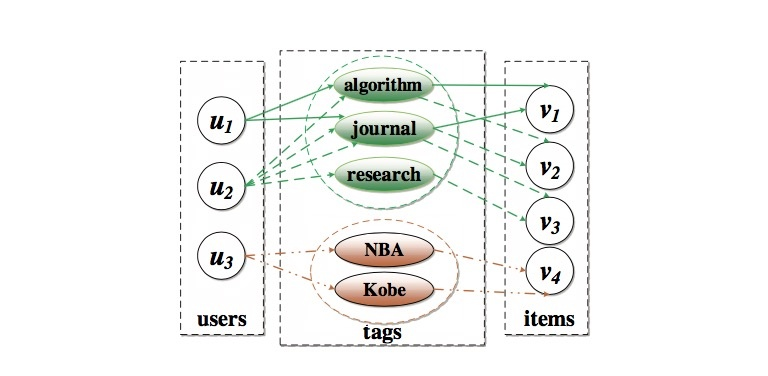
\includegraphics[width=\linewidth]{images/figure1.jpg}
\caption{一个标签系统的例子。每个标签都对应了一个评分,为简洁起见省略了评分。}
\label{fig:fig1}
\end{figure}


这个例子中,用户 $u_1$ 标注了物品 $v_1$,用户 $u_2$ 标注了物品 $v_2$ 和 $ v_3$,因此,用户 $u_1$ 和用户 $u_2$ 之间没有共同评分项。我们定义这种情况为*无共同评分项的稀疏性问题(DS-WO-CRI),DS-WO-CRI 是标准的数据稀疏性问题(在所有的用户物品对中只有很少比例的已知项)的一个典型子集。在 DS-WO-CRI 的情况下,已有的协同过滤方法,例如,PMF 和 CTR 模型,都无法将物品 $v_1$ 推荐给用户 $u_2$ ,因为这些方法无法捕获它们之间的任何联系。然而,一个好的推荐系统应该能够将物品 $v_2$ 和 $v_3$ 推荐给用户 $u_1$ 并且将物品 $v_1$ 推荐给用户 $u_2$,因为在这个例子中,用户 $u_1$ 和 $u_2$ 很可能是算法方面的研究者,而物品 $v_1$, $v_2$ 和 $v_3$ 可能跟算法有关。

现有的研究表明,用户对一个物品的评分或标注等动作就可以表明用户喜好该物品,而不需考虑评分的等级\cite{Koren2008Factorization,Koren2009Matrix}。换句话说,用户通过标记和评分隐式的表达了他的偏好\cite{Koren2008Factorization}。因此,一个用户和他所标注和评分的物品趋向于具有相似的潜在特征,我们在本文中将其定义为隐式偏好(implicit preference)。在上面的例子中,用户 $u_2$ 将物品 $v_3$ 标注为 “journal” 和 “research”,这在表明用户 $u_2$ 可能是一名研究者同时,也指出物品 $v_3$ 可能是一篇学术期刊或其他相关的东西。因此,在语义上,用户 $u_2$ 和物品 $v_3$ 的潜在特征应该具有某种程度的相似。

然而,现有的方法无法捕获用户和物品之间的语义关系,因此它们的推荐性能被局限了,尤其是在 DS-WO-CRI 的情况下。


\textbf{我们的提议}\quad 为了解决上面提到的 DS-WO-CRI 问题,我们在这篇文章中提出了一种新型的协同过滤系统。我们首先利用主题模型依次为每一个用户和每一个物品挖掘标签的语义信息,然后将这些语义信息纳入矩阵分解,同时捕获标签和评分在用户和物品间的桥接特性(即,隐式偏好)。因此,我们的模型可以捕获用户和项目间的语义关联,并将具有相似语义信息的物品推荐给用户,即便是在 DS-WO-CRI 的情况下。

\textbf{贡献}\quad 我们的工作主要有以下贡献:
(1)我们首先指出标签的重要特性,即它们做为桥梁将用户和物品连接起来,概述了用户和物品之间的语义联系,然后我们说明了利用此特性可以帮助解决 DS-WO-CRI 问题。据我们所知,这是首个针对这个问题的研究。
(2)我们提出了一种新型的基于标签和评分的协同过滤模型,它可以捕获用户和物品之间的语义联系,因此可以大大地提升推荐性能,尤其是在 DS-WO-CRI 的情况下。我们还提出了基于坐标上升的参数学习方法。据我们所知,这项研究是文献中对捕获用户和物品语义关联的首次尝试。
(3)在两个流行的真实世界的数据集上的实验表明,我们提出的模型在精确率和召回率方面都显著优于最先进的方法。实验还表明,我们的模型是一个解决 DS-WO-CRI 问题的有效方法。


\chapter{相关工作}
在本节中,我们将分三组来回顾已有的物品推荐方法,其中包括:传统的协同过滤方法、基于主题模型的协同过滤方法、以及基于社交关系的协同过滤方法。

基于已有的研究\cite{shi2014collaborative},传统的协同过滤方法仅利用用户物品的评分进行推荐,主要分为两种类型:基于内存的协同过滤\cite{deshpande2004item}和基于模型的协同过滤\cite{Koren2009Matrix,Koren2008Factorization,Zhou2009TagRec,Xu2015Ice},这两种方法都可以用于标签系统的推荐。

传统的协同过滤方法无法借助文本内容的信息,因此,一些混合模型被提出来,它们结合基于内容的方法和协同过滤方法进行推荐\cite{Melville2002Content}。但是,这些方法简单的将内容表示为词向量的形式,因而无法发掘它们的语义信息。为了利用内容所提供的语义信息,研究者利用主题模型提高推荐效果,Agarwal 等人提出了 fLDA 模型\cite{Agarwal2010fLDA},该方法通过将 LDA 中学习到的先验信息加入物品向量,结合了 RLFM\cite{Agarwal2010fLDA} 和隐式狄利克雷分布(LDA)。RLFM 和 fLDA 都能纳入额外的原信息,例如用户年龄和物品类别,然而,这些附加元特征信息不在本文的范围之内。稍后的,Wang 等人\cite{Wang2011Collaborative} 将概率矩阵分解\cite{Salakhutdinov2008Probabilistic} 与 LDA \cite{Blei2003Latent} 相结合,提出了协同主题回归模型。在\cite{Wang2011Collaborative} 中证明了在相似的情况下 CTR 的性能要优于 fLDA,因为 fLDA 基本忽略了其他用户的评分。

此外,用户之间和物品之间的社会信息对于提升推荐的性能是有效的\cite{Chen2013Recommender}。首先,用户的社会信息被纳入常规的协同过滤模型\cite{Jamali2010A},例如,Ma 等人提出 Soreg 来约束具有联系的用户的潜在因子之间的差异性。之后,相邻用户和物品的社会信息被引入了基于主题模型的协同过滤中以进一步改善推荐性能,例如,Purushotham、Liu 和Kuo \cite{purushotham2012collaborative} 以及 Chen 等人 \cite{Chen2014Context} 提出了两种模型(CTR-SMF 和 CTR-SMF2),将用户社交关系网络纳入CTR,以进一步提高项目推荐性能。Wang、Chen 和 Li \cite{Chen2014Context} 提出了一个将物品的社会关系引入 CTR 的模型,以提高标签系统中的标签推荐性能。


\chapter{提出的模型——TRCF}
在本节中,我们提出一个新的基于标签和评分的协同过滤方法(TRCF)。我们首先正式确定基于标签的物品推荐问题并定义一些符号。然后,我们提出 TRCF ,这是一个分层的贝叶斯模型。最后,我们提出了基于坐标上升的参数学习方法。

\section{初步定义}
假定,我们有一个用户的集合 $U=\{u_1,\dots,u_I \}$,这些用户用一组标签 $T=\{t_1,\dots,t_N \}$ 标记了的一组物品 $V=\{v_1,\dots,v_J \}$,以及评分的集合  $R=\{r_1,\dots,r_O \}$,其中,$I$ 、$J$、$N$ 和 $O$ 依次代表了用户、物品、标签和评分的数目。每一个用户-物品-标签-评分(U-I-T-R)的可观察数据是一个四元组$(u_i, v_j, T_{ij}, R_{ij})$,其中 $u_i \in U$,$v_j \in V$,$T_{ij}$ 是用户 $u_i$ 给予物品 $v_j$ 的标签集合,并且 $T_{ij} \in T$ ,$R_{ij}$ 是用户 $u_i$ 给予物品 $v_j$ 的评分,评分基于用户对该物品的喜好程度并在同时标注它。然而,用户-物品(U-I)的评分集合 $R$ 一般是整数集合,例如,*MovieLens* 使用 [1,5] 范围内的评分。$U \in R^{K*I}$ 表示潜在的用户特征矩阵,其中列向量 $U_i$ 表示属于用户 $u_i$ 的 $K$ 维潜在特征向量。$V \in T^{K*J}$ 表示潜在的物品特征矩阵,其中列向量 $V_j$ 表示属于物品 $v_i$ 的 $K$ 维潜在特征向量。

对于基于标签和评分的物品推荐中,给定现有的四元组 U-I-T-R ,我们的目标是预测用户 $u_i$ 对物品 $v_j$ 的未知的评分。

\section{基于标签和评分的协同过滤}
TRCF 是一个新型的分层的贝叶斯模型,图 \ref{fig:fig2} 展示了它的图模型,其中 $N_u$ 和 $N_v$ 依次表示用户 $u_i$ 和物品 $v_j$ 的标签数目。我们首先将每个用户和物品的标签依次分组,然后使用隐式狄利克雷分布依次对每个用户和每个物品的标签集合进行语义挖掘(图 \ref{fig:fig2} 中以红色绘制)。最后将这些语义信息纳入矩阵分解用于分解评分信息(图 \ref{fig:fig2} 中以紫色绘制)以及捕获标签和评分所提供的隐式偏好(图 \ref{fig:fig2} 中以蓝色绘制)。
\begin{figure}
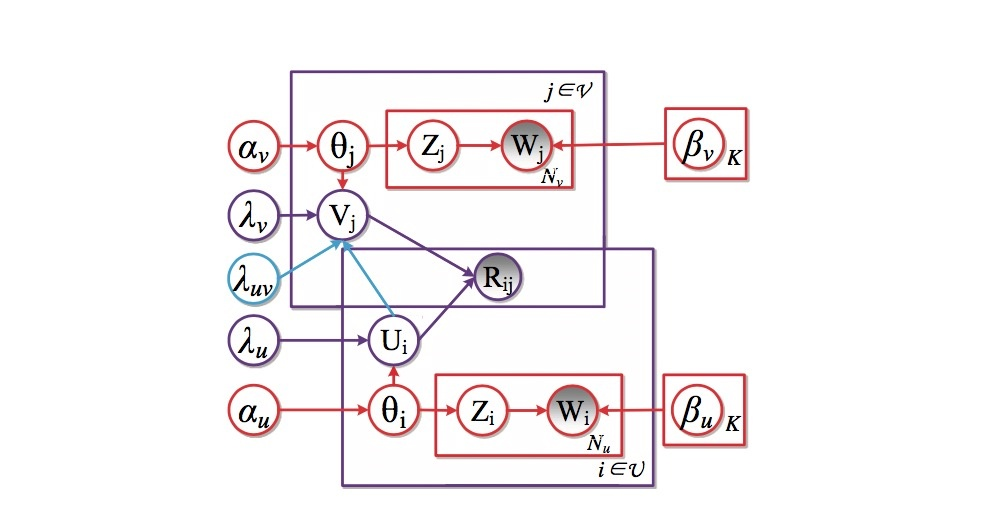
\includegraphics[width=\linewidth]{images/figure2.jpg}
\caption{TRCF 的图模型。LDA 部分以红色绘制,隐式偏好部分以蓝色绘制,PMF 部分以紫色绘制。}
\label{fig:fig2}
\end{figure}

TRCF 同时在用户和物品两个方面上执行 LDA ,因此可以同时捕获用户和物品的语义信息,而不仅仅像现有的工作那样只捕获物品的语义信息。另外,在 TRCF 中,如果一个用户和一个物品通过标签或评分相关联,那么他们的隐式特征会在某些程度上比较相似,这被称为隐式偏好。相比之下,现有的基于主题建模的CF方法,例如,CTR、CTR-SMF 和 CTR-SMF2,都是假设用户和物品是独立的,并且忽略标签和评分在用户和项目之间的桥接作用。因此,TRCF 可以捕获用户和物品之间的语义关联,并且能够处理 DS-WO-CRI 问题。假定每个用户和每个物品都有 $K$ 个主题, TRCF 的执行过程如下:

\begin{enumerate}[itemindent=1em]
	\item \textbf{挖掘用户标签的语义信息。} 对于每个用户 $u_i$ :
	\begin{enumerate}[itemindent=1em]
		\item 选取主题分布 $\theta_i \sim Dirichlet(\alpha_u)$ ;
		\item 选取用户的潜在向量 $U_i \sim \mathcal{N}(\theta_i, \lambda_u^{-1} I_k)$ ;
		\item 对于用户 $u_i$ 的每一个标签 $w_{in_u}$ :
		\begin{enumerate}[itemindent=1em]
			\item 选取主题 $z_{in_u} \sim Mult(\theta_i)$ ;
			\item 选取标签 $w_{in_u} \sim Mult(\beta_{z_{in_u}}) $ ;
		\end{enumerate}
	\end{enumerate}
	\item \textbf{挖掘物品标签的语义信息,并且采集用户和物品间的隐式偏好。} 对于每一个物品 $v_j$ :
	\begin{enumerate}[itemindent=1em]
		\item 选取主题分布 $\theta_j \sim Dirichlet(\alpha_v)$ ;
		\item 选取物品的潜在向量 $V_j \sim \mathcal{N}(\theta_j, \lambda_v^{-1} I_k) \times \prod\limits_{i} I_{ij}^R \mathcal{N}(U_i, \lambda_{uv}^{-1}I_K ) $ ;
		\item 对于物品 $v_j$ 的每一个标签 $w_{jn_v}$ :
		\begin{enumerate}[itemindent=1em]
			\item 选取主题 $z_{jn_v} \sim Mult(\theta_j)$ ;
			\item 选取标签 $w_{jn_v} \sim Mult(\beta_{z_{jn_v}}) $ ;
		\end{enumerate}
	\end{enumerate}
	\item \textbf{获取评分。} 对于每一个用户-物品对 $(i,j)$ :
	$$
		R_{ij} \sim \mathcal(U_i^ T V_j, c_{ij}^{-1}).
	$$
\end{enumerate}

在上面的生成过程中,$\mathcal{N} \sim (x | \mu, \sigma^2)$ 是期望为 $\mu$ 方差为 $\sigma^2$ 的高斯分布,$I_K$ 是一个 $K$ 行 $K$ 列的单位矩阵。$I_{ij}^R$ 是一个指示函数,如果用户 $u_i$ 为物品 $v_j$ 打分了,它的值为 1,否则为 0。$C$ 是评分置信度矩阵,其中的项 $c_{ij}$ 表示评分的置信度。更多细节请参考\cite{Wang2011Collaborative}。

参数 $\lambda_u$ 平衡了用户语义信息提供的标签和评分信息对模型性能的影响。类似地,参数 $\lambda_v$ 平衡了由物品语义信息提供的标签和评分信息对推荐性能的影响。参数 $\lambda_{uv}$ 平衡隐式偏好对模型性能的贡献,即通过评级和标签链接的用户和项目之前潜在特征相似度的程度。

观察到的评分的条件分布可以被形式化为:
$$
p(R | U, V, C) = \prod\limits_i \prod\limits_j \mathcal{N} (R_{ij}|U_i^T V_j,c_{ij}).
$$

用户和物品的潜在向量 $U_i$ 和 $V_j$ 生成的方式与 CTR 相似,它们可以被形式化为:
\begin{equation}
\begin{aligned}
&p(U|\lambda_u) \sim \prod\limits_i \mathcal{N} (\theta_i, \lambda_u^{-1}I_K), \\
&p(V|U, \lambda_v, \lambda_{uv}) \sim  \prod\limits_j \mathcal{N} (\theta_j, \lambda_v^{-1}I_K)  \times \prod\limits_{i} I_{ij}^R \mathcal{N}(U_i, \lambda_{uv}^{-1}I_K ).
\end{aligned}
\end{equation}

给定了 U-I-T-R 信息,通过使用贝叶斯推理,我们可以得到 TRCF 的潜在特征向量的后验概率的如下式子:
\begin{equation}
p(U,V| R,C,\lambda_u, \lambda_v, \lambda_{uv})  \propto p(R | U, V, C) p(U|\lambda_u) p(V|U, \lambda_v, \lambda_{uv}) .  
\label{eq1}
\tag{1}
\end{equation}


\section{TRCF 的参数学习}

给定主体参数 $\beta_u$ 和 $\beta_v$ ,直接计算 $U_i, V_j, \theta_i, \theta_j$ 的完整后验是困难的。我们使用坐标上升的方法来学习最大后验概率。使等式 $\eqref{eq1}$ 中具有固定超参数的两个潜在特征的后验最大化等价于,在给定 $\lambda_u , \lambda_v$ 的条件下, 使如下的 $U, V, \theta_{1:I}, \theta_{1:J}$ 的对数似然函数最大:
\begin{equation}  
\begin{aligned}
L = & -\frac{\lambda_u}{2} \sum\limits_i{ (U_i - \theta_i)^T  (U_i - \theta_i) }  \\ 
	& -\frac{\lambda_v}{2} \sum\limits_j{ (V_j - \theta_j)^T  (V_j - \theta_j)   } \\
	& -\sum\limits_{ij} \frac{c_{ij}}{2} (R_{ij} - U_i^T V_j)^2 \\
	& +\sum\limits_i \sum\limits_{n_u} log \left(\sum\limits_k \theta_{ik} \beta_{k,w_{in_u}} \right) \\
	& +\sum\limits_j \sum\limits_{n_v} log \left(\sum\limits_k \theta_{jk} \beta_{k,w_{jn_v}} \right) \\
	& - -\frac{\lambda_{uv}}{2} I_{ij}^R \sum\limits_{ij} (U_i - V_j)^T (U_i - V_j).  
\end{aligned} 
\label{eq2}
\tag{2}
\end{equation}

我们省略一个常数并设置狄利克雷先验 $\alpha_u = \alpha_v = 1$ 。这个函数可以通过使用坐标上升来优化,也就是说,我们固定 $\beta_u$ 和 $\beta_v$ ,并迭代优化 MF 变量 $U_i , V_j$ 和主题分布 $\theta_i , \theta_j$ 。具体来说,我们首先根据 $\theta_i , \theta_j$ 当前的估计值更新 $U_i$ 和 $V_j$ ,我们计算等式 $\eqref{eq2}$ 中 $L$ 在 $U_i , V_j$  上的导数,并且将它设置为 0 :
\begin{equation}
\label{eq3}
\frac{\partial{L}}{\partial{U_i}}  = 0, \frac{\partial{L}}{\partial{V_j}}  = 0.
\tag{3}
\end{equation}

解决上述的公式得到参数更新的式子:
\begin{equation}  
\begin{aligned}
& U \leftarrow  \left(  VC_iV^T + \lambda_uI_K  + \lambda_{uv}\sum\limits_i I_{ij}^R I_K \right)^{-1}
(VC_iR_i + \lambda_u\theta_i + \lambda_{uv} \sum\limits_j {I_{ij}^R V_j}), \\
& V \leftarrow  \left(  UC_jU^T + \lambda_vI_K  + \lambda_{uv}\sum\limits_i I_{ij}^R I_K \right)^{-1}
(UC_jR_j + \lambda_v\theta_j + \lambda_{uv} \sum\limits_i {I_{ij}^R U_i}).
\end{aligned} 
\label{eq4}
\tag{4}
\end{equation}

其中对于每一个用户 $u_i$ ,$C_i$ 是一个对角矩阵,它的对角元素是 $c_{ij}, j= 1, \dots, J$ ,并且 $R_i = {R_{ij}} _{j=1}^J$ 。对于物品 $v_j$ ,$C_j$ 和 $R_j$ 的定义是相似的。

公式 $\eqref{eq4}$ 显示了参数 $\lambda_u$、$\lambda_v$ 和 $\lambda_{uv}$ 是如何影响用户和物品的潜在特征的。越大的 $\lambda_u$ 会导致用户的潜在特征越依赖于用户标签,而不是评分信息。类似的,较大的 $\lambda_v$ 表示物品的潜在特征来自物品标签的比例更大,而不是评分信息。此外,更大的 $\lambda_{uv}$ 意味着更强的约束,即通过标签和评分链接的用户和项目应当具有类似的潜在特征,即隐式偏好。从公式 $\eqref{eq4}$ 可以看出,概率矩阵分解(PMF)和协同主题回归(CTR)都是 TRCF 的特殊形式。

接下来,给定当前的 MF 变量 $U_i , V_j$ ,我们更新主题分布参数 $\theta_i$ 和 $\theta_j$ 。对于 $\theta_i$ ,我们先定义 $q(z_{in_u} = k) = \phi_{in_uk}$ ,然后分离包含 $\theta_i$ 的用户并应用 Jensen 不等式:
\begin{equation}  
\begin{aligned}
L(\theta_i) &\geq -\frac{\lambda_u}{2}  (U_i - \theta_i)^T  (U_i - \theta_i)  \\
& + \sum\limits_{n_u} \sum\limits_k{ \phi_{in_uk} (log{\theta_{ik} \beta_{k, w_{in_u}}  -  log{\phi_{in_uk}} })}  \\
&=L(\theta_i, \phi_i).
\end{aligned} 
\end{equation}

其中,$\phi_i = {\phi_{in_uk}}_{n_u=1,k=1}^{N_u \times K}$ 。显然 $L(\theta_i, \phi_i)$ 是 $L(\theta_i)$ 的严格下界,因此我们可以使用映射梯度\cite{bertsekas1999nonlinear} 来优化 $\theta_i$ 。最优的 $\phi_{in_uk}$ 正比于 $\theta_{ik} \beta_{k,w_{in_u}}$ 。对于 $\theta_j$ ,更新的规则是相似的。

对于 $\beta_u$ ,我们像 LDA 那样为主题执行 M 步的更新。
$$
\beta_{kw_i} \propto \sum\limits_i \sum\limits_{n_u} \phi_{in_uk} 1 [w_{in_u} = w].
$$

对于 $\beta_v$ ,它的更新策略是相似的。当参数 $U^*, V^*, {\theta_{1:I}}^*,  {\theta_{1:J}}^* , {\beta_u}^*, {\beta_v}^*$ 的最优值学习完成后,我们的模型就可以进行评分预测了:
$$
{R_{ij}}^* \approx ({U_i^*})^T V_j^*.
$$


\chapter{实验和分析}
在本节中,我们介绍了对两个流行的现实世界数据集进行的实验,目的是回答如下的问题:(1)我们的模型相比现有的最先进的方法有什么改进? (2)我们的方法如何处理 DS-WO-CRI 问题? (3)参数 $\lambda_u$ ,$\lambda_v$ 和 $\lambda_{uv}$ 如何影响 TRCF 的性能?

\section{数据集}
我们在实验中使用了两个现实世界的数据集:hetrec2011-delicious-2k (Delicious) 和 hetrec2011-lastfm-2k (Lastfm)\cite{Cantador2011Second}。这两个数据集已广泛用于标签系统的实验\cite{Bellog2013A},它们在表 \ref{table1} 中描述。

\begin{table}[]
\centering
\caption{数据集描述}
\label{table1}
\begin{tabular}{@{}cccccc@{}}
\toprule
数据集       & 用户   & 物品    & 标签    & 用户-标签-物品 & 评分     \\ \midrule
Delicious & 1867 & 69226 & 53388 & 437593   & 104799 \\
LastFm    & 1892 & 17632 & 11946 & 186479   & 92834  \\ \bottomrule
\end{tabular}
\end{table}

对于每个数据集,如果用户已将该项目设为书签(或收听),则我们认为该项目的用户评分为 1 ,否则,该项目的用户评分为 0 。

在我们的实验中,我们将每个数据集分为三个部分——训练数据集(80%),留出验证数据集(10%)和测试数据集(10%)。 我们在训练数据集上训练我们的模型,在验证数据集上获得最佳参数,并在测试数据集上评估我们的模型。

\section{比较与评估}
如相关工作中所述,存在许多种推荐方法,例如,基于存储的方法和混合方法。这里,我们将所提出的 TRCF 与以下三种现有的方法进行比较,即常规的协同过滤方法,基于社会关系的 CF 方法和基于主题建模的方法:

% \begin{enumerate}[itemindent=1em]
% \item SVD ++(Koren, 2008)是一种经典的协同过滤方法,该方法仅使用 U-I 评分信息。
% \item Soreg(Ma et al., 2011)是基于社会关系的 CF 方法,其使用 U-I 评分和用户社交信息。
% \item CTR (Wang and Blei, 2011)是一种最先进的基于主题建模的 CF 方法,其使用类似于 TRCF 中使用的四元组 U-I-T-R 的信息。
% \item CTR-SMF(Purushotham, Liu, and Kuo, 2012)结合了用户社交矩阵分解和 CTR 。 它包含除了在 TRCF 中使用的四元组 U-I-T-R 之外的附加用户社交信息。
% \item CTR-SMF2(Chen et al., 2014)改进了 CTR-SMF ,它还将用户社交信息引入了 TRCF 中的 U-I-T-R 四元组。
% \end{enumerate}

\textbf{SVD ++} \cite{Koren2008Factorization} 是一种经典的协同过滤方法,该方法仅使用 U-I 评分信息。

\textbf{Soreg} \cite{Ma2011Recommender} 是基于社会关系的 CF 方法,其使用 U-I 评分和用户社交信息。

\textbf{CTR} \cite{Wang2011Collaborative} 是一种最先进的基于主题建模的 CF 方法,其使用类似于 TRCF 中使用的四元组 U-I-T-R 的信息。

\textbf{CTR-SMF} \cite{purushotham2012collaborative} 结合了用户社交矩阵分解和 CTR 。 它包含除了在 TRCF 中使用的四元组 U-I-T-R 之外的附加用户社交信息。

\textbf{CTR-SMF2} \cite{Chen2014Context} 改进了 CTR-SMF ,它还将用户社交信息引入了 TRCF 中的 U-I-T-R 四元组。

精确率和召回率已被广泛用作评估推荐效果的指标\cite{herlocker2004evaluating}。 因此,我们使用 Precision 和 Recall 来评估推荐性能,并且计算召回率的方式也用于 CTR,CTR-SMF 和 CTR-SMF2。 对于每个用户,Precision 和 Recall 定义如下:
\begin{equation}
\begin{aligned}
Precision@M = \frac{\# \text{Top M 中用户喜欢的物品}}{M},  \\
Recall@M = \frac{\# \text{Top M 中用户喜欢的物品}} {\# \text{用户喜欢的所有物品}}, 
\end{aligned}
\end{equation}
其中 M 是推荐列表中的物品数。 我们计算测试数据集中所有项的精确率和召回率的平均值作为最终结果。

\section{性能对比和分析}
在对比不同模型时,我们使用在 CTR-SMF \cite{purushotham2012collaborative} 中设置的 SVD++、CTR 和 CTR-SMF 的最佳参数,它们使用相同的数据集。 对于 Soreg、CTR-SMF2 和我们的模型,我们使用网格搜索来获得最佳参数。
\begin{figure}
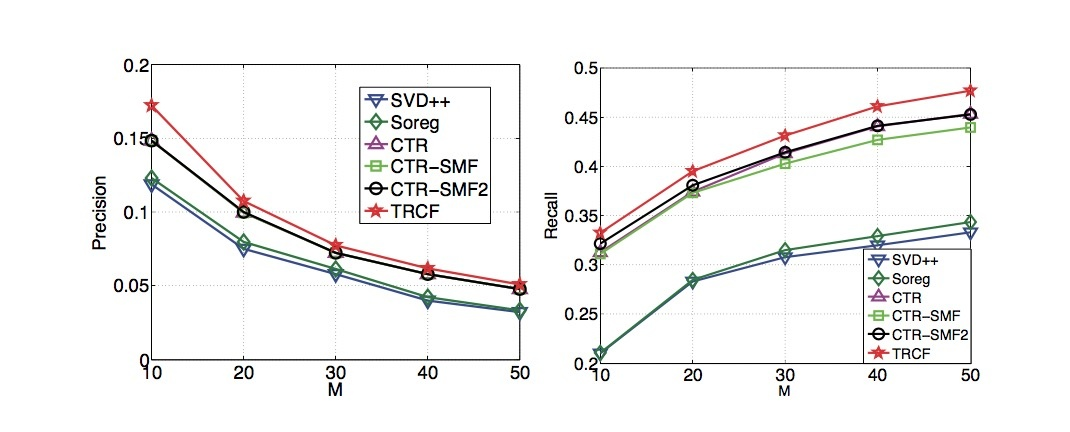
\includegraphics[width=\linewidth]{images/figure3.jpg}
\caption{在 Delicious 数据集下设置不同的 M 值,精确率和召回率的对比,以及每个方法的最优参数}
\label{fig:fig3}
\end{figure}
\begin{figure}
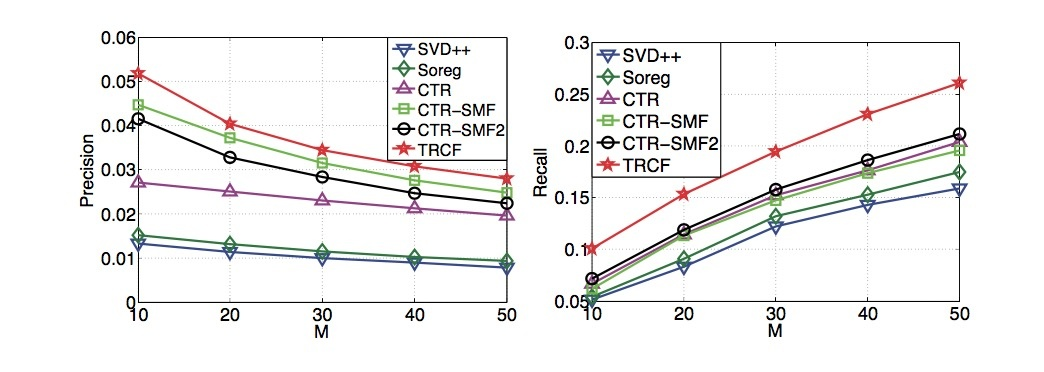
\includegraphics[width=\linewidth]{images/figure4.jpg}
\caption{在 LastFm 数据集下设置不同的 M 值,精确率和召回率的对比,以及每个方法的最优参数}
\label{fig:fig4}
\end{figure}


\textbf{结果:} 图 \ref{fig:fig3} 和图 \ref{fig:fig4} 显示了各个推荐方法在 Delicious 数据集和 Lastfm 数据集上的总体性能,其中我们设置 $M = 10,20,30,40,50$ 并将每个方法的参数固定为最佳值。 结果表明,传统的 CF 方法(SVD ++)和基于社交关系的 CF 方法(即 Soreg)具有相似的性能。 三个基于主题建模的 CF 方法(即 CTR、CTR-SMF 和 CTR-SMF2)具有类似的性能,并且显著优于 SVD++ 和 Soreg,这表明了标签信息在推荐中的重要性。

我们提出的 TRCF 方法在这两个数据集上显著优于 SVD++、Soreg、CTR、CTR-SMF 和 CTR-SMF2。具体在平均值上,在 Delicious 数据集上,TRCF 在精确度方面将 SVD++、Soreg、CTR、CTR-SMF 和 CTR-SMF2 提升了 46.75%、39.74%、8.62%、8.78% 和 8.65%,并且在召回率方面分别提高了 44.99%、42.40%、5.23%、7.27% 和 4.21% 。在 Lastfm 数据集上,TRCF 在精确度方面将 SVD++、Soreg、CTR、CTR-SMF 和 CTR-SMF2 提升了 259.80%、210.27%、57.96%、11.64% 和 23.85% ,并且在召回率方面分别提高了 73.03%、60.39%、34.18%、39.04% 和 28.12% 。


\textbf{分析和总结:} 以上的对比表明了我们提出模型的有效性,它捕获了用户和物品之间的语义关联。实验结果表明,尽管用户的社交信息可以改善推荐性能,但是改善推荐性能的更有效的方式是考虑用户和物品的语义相关性。


\section{DS-WO-CRI 实验}
所有四种基于主题建模的 CF 方法(包括 TRCF)都可以通过采集物品的语义信息来提高推荐性能。为了研究它们处理 DS-WO-CRI 问题的能力,我们进行以下实验。我们首先依据 DS-WO-CRI 的程度将 LastFm 数据集分为四个子数据集,每个数据集在表 2 中描述了。DS-WO-CRI 的程度定义如下:
$$
x\% = \frac{\#\text{没有共同评分物品的用户数目}}{\#\text{总的用户数目}}.
$$
然后我们对每个子数据集进行对照实验。图 \ref{fig:fig5} 显示,我们的模型在不同的 DS-WO-CRI 程度下都达到最佳性能。我们的模型相对于其他三个主题建模方法的在 LC1、LC2、LC3、LC4 上精确率的平均改进分别为 49.67%、75.81%、345.77% 和 428.97% ,召回率的改进分别为 33.94%、65.00%、383.63 % 和 458.00% 。实验结果表明,DS-WO-CRI 的程度越严重,我们的模型相对其它模型的优势越明显。
\begin{figure}
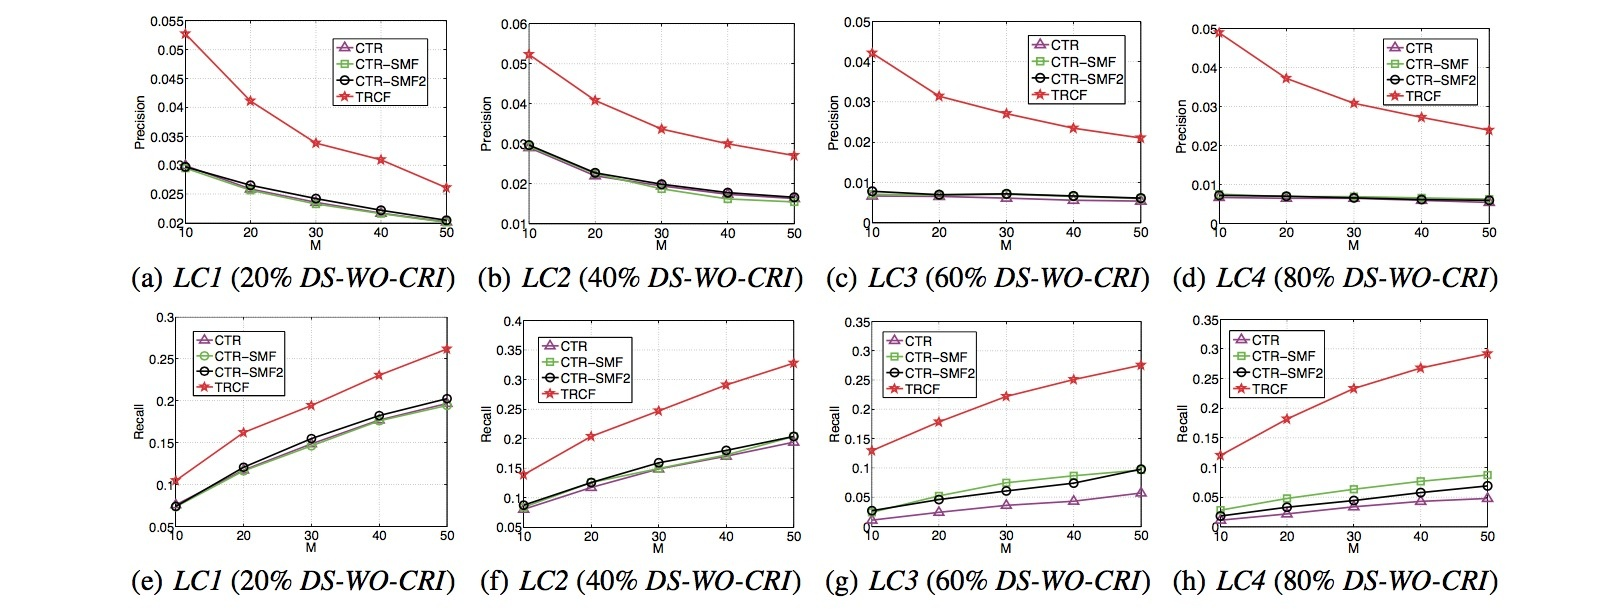
\includegraphics[width=\linewidth]{images/figure5.jpg}
\caption{在每个 DS-WO-CRI 子数据集上设置每种方法的最优参数,精确率和召回率对比。}
\label{fig:fig5}
\end{figure}

\textbf{总结:} DS-WO-CRI 实验表明了我们提出的模型在处理该问题时的有效性:越严重的 DS-WO-CRI 情况,我们的模型相比其它模型的优势越明显。这是由于我们的方法具有采集用户和物品间标签语义关联的能力。


\section{参数影响}
图 \ref{fig:fig6:a} 显示了在 LastFm 数据集上固定公式 $\eqref{eq2}$ 中的参数 $\lambda_{uv} $ 时, 参数 $\lambda_u$ 和 $\lambda_v$ 对 TRCF 性能的影响。我们可以看到,当 $\lambda_u = \lambda_v = 10$ 时,TRCF 达到最佳性能,这说明用户和物品语义信息都对模型性能有显着的贡献。图 \ref{fig:fig6:b} 显示了在四个 DS-WO-CRI 子数据集上固定 $\lambda_u$ 和 $\lambda_v$ 为最佳值时,公式 $\eqref{eq2}$ 中的参数 $\lambda_{uv} $ 对 TRCF 性能的影响。我们可以看到,TRCF 的性能首先随着 $\lambda_{uv} $ 的增大而上升,然后在某个阈值后开始下降。在 LC1、LC2、LC3、LC4 上最佳的 $\lambda_{uv}$ 值分别是 0.0001、0.01、0.01 和 0.1。这个结果说明了 DS-WO-CRI 的程度越大,对应的 $\lambda_{uv}$ 的最优值相应的越大。换句话来说,当 DS-WO-CRI 的问题越严重时,通过标签和评分(即隐式偏好)桥接用户和物品的特性越重要,这就解释了为什么我们的模型在可以在严重的 DS-WO-CRI 的情况下表现良好的原因。


\begin{figure}
\centering
\subfigure[$\lambda_u, \lambda_v$ 的影响]{
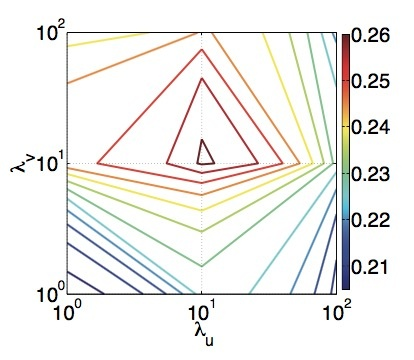
\includegraphics[width=0.45\linewidth]{images/figure6a.jpg}
\label{fig:fig6:a}
}
\subfigure[$\lambda_{uv}$ 的影响]{
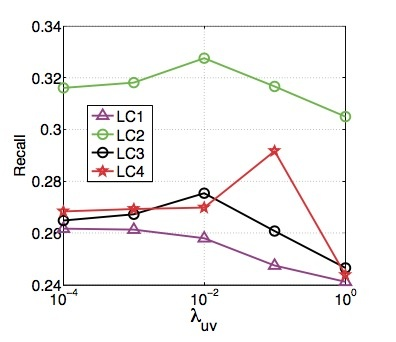
\includegraphics[width=0.45\linewidth]{images/figure6b.jpg}
\label{fig:fig6:b}
}
\caption{固定 M=50, $\lambda_u, \lambda_v, \lambda_{uv}$ 对 TRCF 召回率的影响。}
\end{figure}



\chapter{总结}
在本文中,我们首先介绍了在实际的标记系统中存在的 DS-WO-CRI 问题。 然后,我们提出一个新型的基于标签和评分的 CF 模型来处理这个问题。该模型使用主题建模来分别挖掘用户和物品的标签的语义信息,并将语义信息结合到矩阵分解中以对评分信息进行因式分解,并捕获用户与物品之间的标签和评分的桥接特征 。据我们所知,这是文献中首次尝试引入 DS-WO-CRI 问题并提出一个处理它的模型。 最后,对两个流行的数据集进行的实验表明,我们的模型在精确率和召回率方面显着优于目前最先进的方法,特别是在 DS-WO-CRI 情况下。

\chapter{致谢}
我们感谢匿名审稿人的有益建议。这项工作得到了中国国家自然科学基金(61379034)、国家重点技术研发计划(2014BAH28F05)、广东省科技计划(2013B040100004, 2013B040403002)和中国浙江省自然科学基金(LQ14F010006)的部分支持。


\bibliography{data/文献翻译}






 

%==============================================================
%这也是个不需要自己修改的部分。

  \backmatter %结束章节自动编号

%==============================================================


\end{document}
